\chapter{慢性关节痛}

随着抗生素的广泛使用,感染性关节炎和感染相关的关节炎已明显减少。而今绝大多数关节炎属于慢性关节炎,即使是以急性关节炎起病,最终多是转归为慢性关节炎,或是可以出现反复急性发作的慢性关节炎。因此,学习关节炎的鉴别诊断应重点放在这一章。

骨关节疼痛是一常见的临床症状。骨关节疼痛是风湿病的主要表现,但也可见于非风湿病者。风湿病包括自身免疫性和非自身免疫性,而非风湿病的骨关节疼痛则包括肿瘤性、感染性、内分泌性、神经性、功能性等等。

\section{【症状学与人口学特征】}

从症状学的特征尤其是骨关节疼痛的规律和特征,在很大程度上可以判断病变的性质。从发病年龄、性别等人口学特征,可以帮助判断患某病的概率,多考虑什么,少考虑什么。所以,当接诊关节炎患者时,首先需要从症状学和人口学特征开始建立鉴别诊断思路。

\subsection{(一)晨僵现象与关节痛的昼夜规律}

晨僵现象与关节痛的昼夜规律在关节炎的鉴别诊断中非常重要。晨僵者往往主诉下半夜和(或)早晨起床时关节疼痛、僵硬或不适症状加重,起床活动后逐渐减轻。晨僵现象的持续时间,短则十几分钟,长则大半天。

有明显晨僵者往往提示该关节疼痛是炎症性的,多是与自身免疫相关的风湿病,即传统概念中的结缔组织病,如类风湿关节炎、血清阴性脊柱关节病(强直性脊柱炎等)、系统性红斑狼疮、系统性硬化症、风湿性多肌痛等。

骨关节炎多无晨僵,特殊类型的骨关节炎(手指出现Heberden结节和Bouchard结节者)和出现继发性滑膜炎时可有晨僵,但晨僵的时间短暂,一般不超过30分钟。非风湿病的疼痛(如外伤、神经性疼痛等)一般无晨僵。

\subsection{(二)关节肿胀}

关节肿胀提示疾病活动期。按压有波动感提示有关节腔积液。手指关节按压柔韧感提示滑膜增厚,关节肿胀可见于各种炎症性关节病变,如类风湿关节炎、强直性脊柱炎的下肢大关节、继发滑膜炎的骨关节炎、痛风等。

肿胀和压痛部位在关节的边缘或上、下方,提示肌腱骨附着点炎症,是血清阴性脊柱关节病(如强直性脊柱炎、莱特尔综合征等)的特征。

\subsection{(三)疼痛与活动的关系}

活动后症状减轻,提示是自身免疫介导的炎症性病变。活动后症状加重,则提示是退行性病变(如骨关节炎)或机械性因素(如椎间盘突出)导致的疼痛。

关节疼痛休息不能缓解,长时间不活动反而更痛或僵硬,则提示免疫介导的风湿病,如类风湿关节炎、血清阴性脊柱关节病。骨关节炎的疼痛则多发生在活动时,如行走、上下楼梯、爬坡等症状加重,休息后好转。

\subsection{(四)关节肿痛的持续时间与“游走性关节炎”的关系}

关节肿痛超过6周者,需要考虑侵蚀性风湿病,如类风湿关节炎、血清阴性脊柱关节病,也需排除肿瘤和感染性关节炎。继发滑膜炎的骨关节炎的关节肿胀多持续1~3周,少数严重者也可超过6周。

红斑狼疮的关节痛可以是固定的,也可以是游走性。风湿热的多关节炎呈游走性。所谓游走性是指各个关节肿痛此起彼伏,某个肿痛的关节持续数小时至数天后自然消退。需要注意的是,血清阴性脊柱关节病的外周关节肿痛常常是不对称的和变换部位的,可以是“今年左踝关节肿痛,明年右膝关节肿痛,再过几个月又左膝关节肿痛”等等,每个部位的疼痛持续时间为数周至数月,而局部X线片往往阴性。许多非风湿病专科的医生将此误认为是“游走性”和“非侵蚀性”关节炎,而误诊为多关节炎的风湿热。

\subsection{(五)年龄与性别}

青少年男、女注意风湿热,青少年男性多注意强直性脊柱炎;青壮年女性多注意系统性红斑狼疮,青壮年男性多注意莱特尔综合征;中老年男性痛风常见,中老年女性骨关节炎常见。40岁以后起病者极少强直性脊柱炎。生育年龄的女性极少痛风,因为雌性激素可以促进尿酸的排泄,因此女性痛风主要见于更年期以后。中年女性主诉浑身疼痛,需考虑到纤维织炎(纤维肌痛症)。

\section{【病变部位】}

\subsection{(一)中轴骨关节}

累及脊柱的风湿病主要是血清阴性脊柱关节病(强直性脊柱炎等)、骨关节炎等。

\subsubsection{1.强直性脊柱炎}

主要是下腰部、颈部疼痛,颈椎、腰椎受累表现为颈部活动和弯腰受限;胸椎受累早期为胸闷、胸痛,后期表现为胸廓活动度下降;骶髂关节损害是强直性脊柱炎的早期表现、确诊条件和鉴别诊断的关键。但由于骶髂关节在平时是不活动性关节,多数骶髂关节炎仅表现为轻度酸胀或胀痛,较少成为患者的主诉。

多数强直性脊柱炎就诊时的主诉是腰痛、颈痛、肩痛、髋痛、下肢大关节痛或足跟痛,临床医生在给患者申请放射学检查时,往往只注意检查主诉的疼痛部位,而忽略了骶髂关节。结果患者花了不少钱,照了许多片(包括X线平片、CT、MRI等),却不能确诊。因为强直性脊柱炎在起病初期的几年内,这些部位多无明显的放射学改变,或仅表现出轻度骨质增生。

特别是以外周关节炎开始发病的,24\%~75\%的强直性脊柱炎患者在病初或病程中出现外周关节病变,以膝、髋、踝和肩关节居多,肘、手和足小关节偶见受累。非对称性、少数关节或单关节,以及下肢大关节的关节炎为本病外周关节炎的特征,这类患者更易误诊。

有放射学改变的骶髂关节炎却由于不构成患者的主诉而被临床医生忽略,这是强直性脊柱炎常常被误诊和漏诊的主要原因之一。

\subsubsection{2.脊柱骨关节炎}

颈椎受累比较常见。可有椎体、椎间盘以及后突关节的增生和骨赘,引起局部疼痛和僵硬感,压迫局部血管和神经时可出现相应的放射痛和神经症状。颈椎受累压迫椎-基底动脉,引起脑供血不足的症状。腰椎骨质增生导致椎管狭窄时可出现间歇性跛行以及马尾综合征。

外伤等也常引起脊柱病变,如椎间盘脱出、压缩性骨折等。少见的脊柱疼痛的病因包括脊椎结核、肿瘤等,患者一般有原发病的相应表现和放射学的改变。

\subsection{(二)手部关节}

\subsubsection{1.类风湿关节炎}

90\%以上的类风湿关节炎在病程中会累及这三组关节的至少一组:腕、掌指关节和近端指间关节,临床上常将这三组关节称为类风湿关节炎的“靶关节”。受累的指间关节呈梭形肿胀,后期关节变形、脱位可出现掌指关节的尺侧偏斜、手指的天鹅颈畸形等。早期一般不累及远端指间关节。类风湿关节炎所侵犯的关节多为有滑膜组织的可活动关节,脊柱关节中除颈椎有滑膜可受累外,极少累及胸、腰及骶髂关节。

\subsubsection{2.骨关节炎}

手指的骨关节炎则主要累及远端指间关节(Heberden结节)、近端指间关节(Bouchard结节)或第一腕掌关节,极少累及掌指关节和整个腕关节。受累的指间关节在关节背面两侧出现结节样改变。

银屑病关节炎也常累及远端指间关节,但多伴有甲周皮肤或指甲的损害,大部分病例全身皮肤可找到典型银屑病的皮肤改变。

另外,系统性硬化症、莱特尔综合征、痛风、肺性骨关节病等也常累及手部骨关节。

单独一个肘关节疼痛,多考虑网球肘,在其肱骨外上髁有一明确定位的压痛点。各种风湿病都可累及肘关节,但很少单独累及肘关节。结合患者病史、体征及职业等可得出诊断。

\subsection{(三)肩关节}

单独一个肩关节疼痛,多考虑肩周炎。其他各种风湿病都可累及肩关节,但很少单独累及一个肩关节。青少年双肩关节疼痛,多注意强直性脊柱炎;老年的双肩关节疼痛,要注意风湿性多肌痛。

\subsection{(四)下肢关节}

青少年男性下肢大关节不明原因的肿痛,而局部X线检查阴性者,应注意强直性脊柱炎,建议检查骶髂关节。

\subsubsection{1.髋关节}

最常引起髋关节病变的是强直性脊柱炎,而导致强直性脊柱炎致残最关键的关节也是髋关节。对于已确诊的强直性脊柱炎,需要询问和追踪髋关节的症状以及必要的放射学检查,有髋关节损害的强直性脊柱炎,在治疗用药方面需要更加积极一些。在青少年男性以髋关节疼痛为主诉者,首先要注意强直性脊柱炎,注意寻找其他支持点,如查HLA-B27、骶髂关节或脊柱症状、晨僵现象等等。

对于单个髋关节病变者则要注意髋关节结核,髋关节是继胸椎之后骨关节结核的好发部位。临床上会遇到一些单个髋关节病变者,很难鉴别是结核性还是免疫性。关节镜检查虽然很有帮助,但也常见一些病例做完关节镜检查后,关节镜操作者和病理科均无法明确判断是否结核。此时,还有两个方面的资料可以参考,一是髋关节MRI检查,如果周围软组织明显肿胀者,支持结核;二是密切随访,1~3个月内有明显的放射学损害进展者为结核。

激素治疗等原因可引起股骨头缺血性坏死。股骨头缺血性坏死者多主诉髋关节不适,而疼痛多不严重。

\subsubsection{2.膝关节}

膝关节疼痛很常见,几乎所有的关节疾病都可累及膝关节,临床上应根据所伴随的各种特征加以鉴别。老年的膝关节疼痛,最常见于骨关节炎;青少年膝关节疼痛,需注意强直性脊柱炎。

\subsubsection{3.踝关节和足跟}

各种风湿病都可累及踝关节。而足跟的骨刺样疼痛在老年考虑骨质增生,在青壮年考虑血清阴性脊柱关节病。

\subsubsection{4.跖趾关节}

第一跖趾关节红、肿、热、痛应考虑痛风。现代女性的第一跖趾关节疼痛应考虑骨关节炎。类风湿关节炎、莱特尔综合征、银屑病关节炎等也常引起足趾小关节损害。

\subsection{(五)全身性疼痛}

全身关节肌腱疼痛,而一般体检和实验室检查阴性,应考虑纤维织炎(纤维肌痛症),多见于女性,有特异性的压痛点,常伴有睡眠欠安、主诉甚多等症状。全身骨骼疼痛者注意多发性骨髓瘤或转移癌。骨关节炎、系统性红斑狼疮和类风湿关节炎等风湿病也常出现全身多关节肿痛。全身关节痛伴发热、皮疹,且三者平行消长者,应注意成人Still病。

\section{【实验室检查】}

\subsection{(一)炎症指标}

血沉与C反应蛋白增高提示关节病变属炎症性,但无法鉴别是哪一种炎症,治疗后下降提示抗炎有效。骨关节炎在一般情况下血沉与C反应蛋白不增高,若增高则常提示可能继发滑膜炎。

\subsection{(二)非特异性免疫指标}

IgA、IgG、IgM和血清蛋白电泳可提示病变的发生、发展是否有免疫学异常参与,对评估预后和监测疾病活动性有意义。

\subsection{(三)有鉴别诊断意义的指标}

\subsubsection{1.抗核抗体谱}

抗核抗体阳性提示结缔组织病,多见于系统性红斑狼疮、混合性结缔组织病等;抗ds-DNA抗体是系统性红斑狼疮的特异性抗体;抗Sm抗体是系统性红斑狼疮的标记抗体;抗RNP抗体对混合性结缔组织病有重要意义;抗SSA抗体和抗SSB抗体提示干燥综合征;抗Jo-1抗体是多发性肌炎和皮肌炎的标记抗体;抗Scl-70抗体是系统性硬化症的标记抗体。

\subsubsection{2.类风湿因子}

类风湿因子滴度对类风湿关节炎有意义,滴度愈高意义愈大;类风湿因子阳性也见于红斑狼疮、混合性结缔组织病、干燥综合征、系统性硬化症等;少数正常人(约5\%)可出现类风湿因子阳性,老年人阳性率更高些。所以临床上不可将关节痛与类风湿因子阳性的组合盲目地诊断类风湿关节炎。另外,类风湿因子滴度下降两个倍数级才表示抗风湿治疗有效,无滴度的类风湿因子阳性和阴性没有临床指导意义。

\subsubsection{3.抗链球菌溶血素“O”试验}

大于500单位为阳性,提示近期曾有链球菌感染,对诊断风湿热有辅助意义。

\subsubsection{4.抗中性粒细胞胞浆抗体}

对系统性血管炎有重要意义。

\subsubsection{5.其他自身抗体}

抗细胞膜DNA自身抗体(抗mDNA)和抗核小体抗体(AnuA)等对SLE诊断较有意义,AnuA主要的临床意义在于它出现在SLE早期,并与疾病活动性密切相关;抗CCP抗体用于类风湿关节炎(RA)临床的早期诊断,该抗体阳性的RA患者骨关节破坏程度较阴性者严重;以免疫球蛋白结合蛋白(BiP)为靶分子的抗体可见于RF阴性的RA患者,被认为是RA血清诊断标志之一。

\section{【关节滑液检查】}

非炎症性滑液黏滞性高,黄色透明,白细胞<2×10\textsuperscript{6}
/L,中性粒细胞<25\%,葡萄糖含量与血糖相等;炎症性滑液黏滞性低,黄色半透明,白细胞>2×10\textsuperscript{6}
/L,中性粒细胞>50\%,葡萄糖含量明显低于血糖。类风湿关节炎的滑液补体水平低下,而血清补体正常;系统性红斑狼疮的滑液和血清补体水平均低下;而血清阴性脊柱关节病的滑液补体水平多正常或增高。

\section{【放射学检查】}

X线检查是关节疼痛的鉴别诊断中必不可少的项目。强直性脊柱炎需借助骶髂关节照片才能确诊;诊断骨关节炎也需要X线的证据;类风湿关节炎的定期X线检查,可有助于了解病变的进展,客观评价疗效。CT和MRI显像明显较X线平片清晰,更有利于早期诊断。

慢性关节痛疾病的分类见表\ref{tab43-1}。

\begin{table}[htbp]
\centering
\caption{慢性关节痛疾病的分类}
\label{tab43-1}
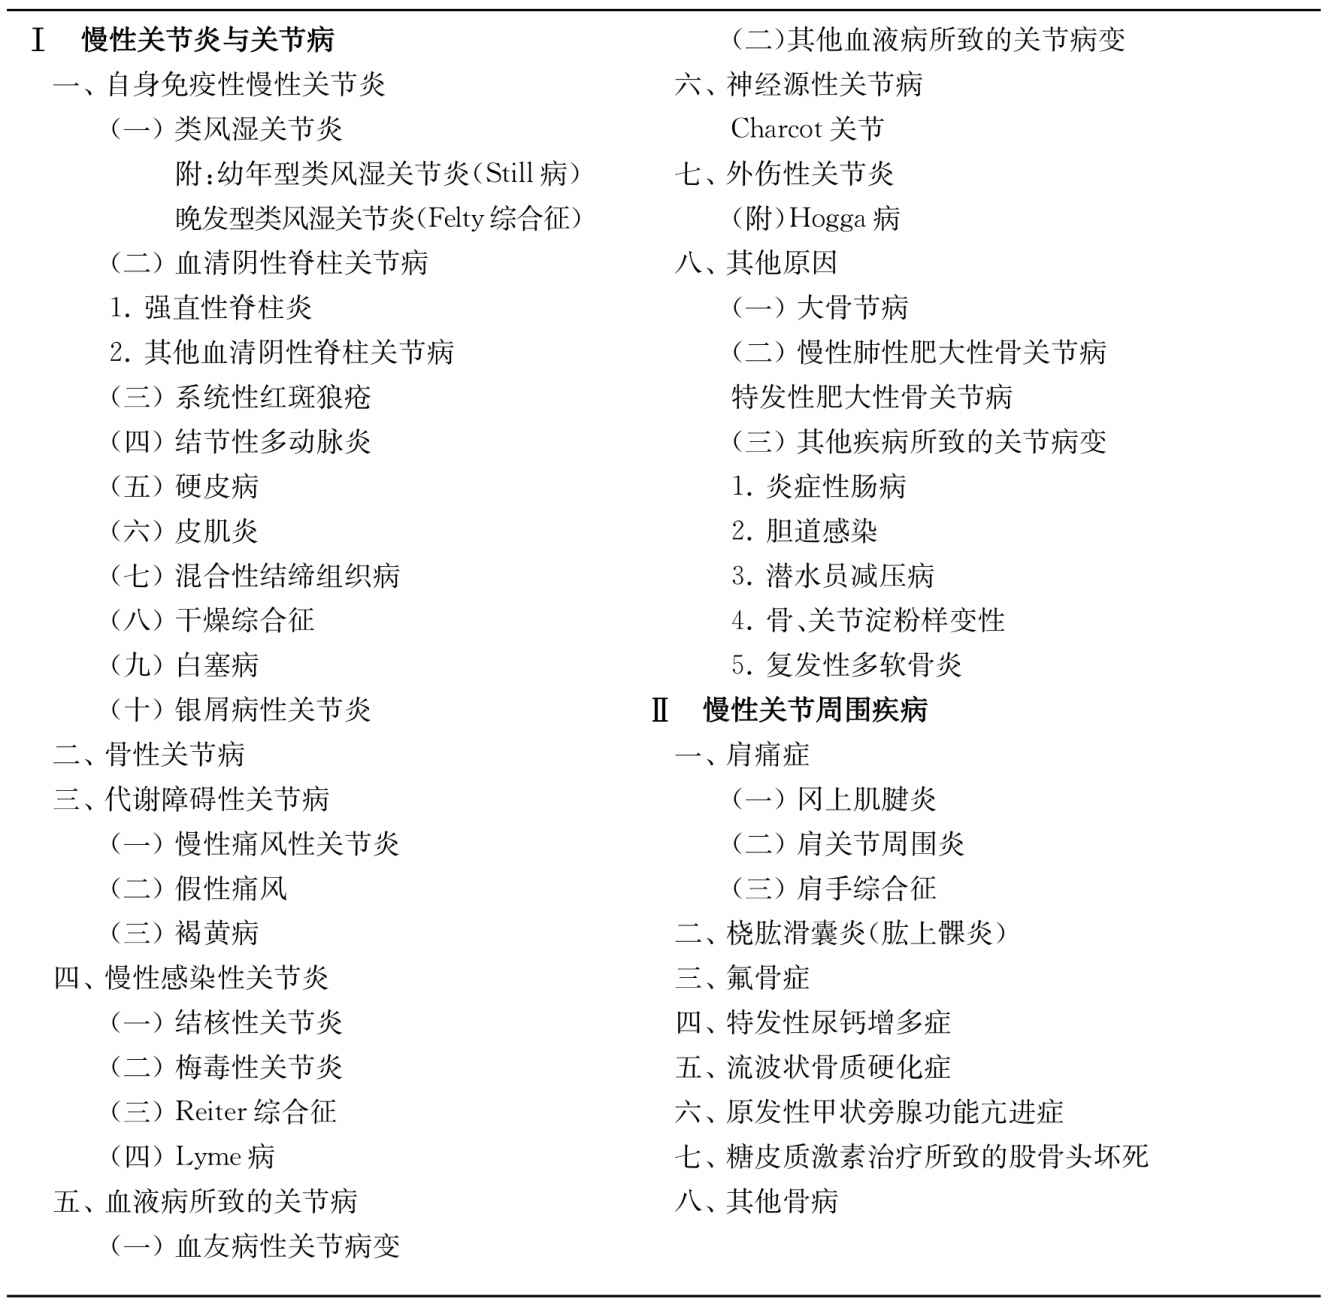
\includegraphics[width=5.89583in,height=5.79167in]{./images/Image00256.jpg}
\end{table}

\protect\hypertarget{text00329.html}{}{}

\section{143 慢性关节炎与关节病}

\subsection{一、自身免疫性慢性关节炎}

\subsubsection{(一)类风湿关节炎}

类风湿关节炎是常见的慢性关节疾病,女性多见,30~50岁为发病高峰,一般呈隐袭性起病,先有几周到数月的乏力、食欲缺乏、体重减轻、低热、手足麻木等前驱症状,部分患者起病急骤,于数日或数周内出现显著的关节症状。类风湿关节炎以双手腕关节、掌指关节和近端指间关节的对称性关节炎为特征性表现。95\%以上的患者在疾病过程中会累及这三组关节的至少一组,所以这三组关节也被称为类风湿关节炎的靶关节。

类风湿关节炎起病急缓不一,多数从手、足小关节开始,尤其是近端指间关节开始发生疼痛、肿胀,并形成对称性梭形指,继而向上发展,渐累及掌指、腕、肘及踝、膝等关节。全身关节均可受累,少数患者因下颌关节或颞颌关节疼痛致张口困难。关节炎症反复发作,终致发生畸形、脱位和强直。形成几个典型类风湿关节炎的关节畸形:掌指关节半脱位形成“尺侧偏斜”;近端指间关节屈曲、远端指间关节过伸形成“纽扣花畸形”;近端指间关节过伸、远端指间关节屈曲形成“天鹅颈畸形”。

约有10\%的病例出现皮下结节,称为类风湿结节。类风湿结节需要与风湿热的皮下结节相鉴别。类风湿结节多位于腕、肘和指部伸侧,花生米大小,质硬,持续时间长,结节内有特殊的局灶性肉芽组织改变;风湿热的皮下结节较小,帽针头大至黄豆大,常见于鹰嘴突、髌骨等处,依附在腱鞘、筋膜上,多见于小儿,治疗后迅速消退。

部分病史长或老年类风湿关节炎患者可伴有低色素性贫血。活动期类风湿关节炎多有血沉和C反应蛋白增高。类风湿因子(RF)测定对诊断类风湿关节炎有重要意义,阳性率达70\%以上,类风湿因子滴度愈高,诊断意义愈大。但是类风湿因子对类风湿关节炎的特异性不高,系统性红斑狼疮、干燥综合征、混合性结缔组织病等也常常出现类风湿因子增高。类风湿因子只是类风湿关节炎的诊断指标之一,不是必备指标,所以临床上不可因类风湿因子阴性而排除类风湿关节炎的诊断。

对于早期不典型的类风湿关节炎患者可行以下自身抗体的检查:

1.抗角蛋白抗体(AKA)
AKA在早期RA,甚至在出现临床症状之前数年就可查出。见于34\%RF阴性的患者。它是类风湿关节炎最特异的标记物,特异性高达80\%~100\%,但敏感性较差,仅有25\%~59\%的患者阳性。AKA与RA病情严重程度和活动性有一定关系。

2.抗核周因子抗体(APF)
特异性不及AKA,但敏感性较好,见于49\%~91\%的患者。与AKA相似,也用于早期、不典型患者的诊断。

3.抗RA-33抗体 敏感性为35\%~45\%,特异性为90\%。

4.抗Sa抗体
RA的另一种特异性自身抗体,敏感性为32\%~43\%。在有关节破坏的RA患者中,此抗体的阳性率可达68\%。见于27\%RF阴性RA患者。

5.抗环瓜氨酸肽抗体(抗CCP抗体)对RA的敏感性为46\%,特异性为90\%以上。此抗体可在关节炎早期出现,并与骨关节的破坏相关。

X线检查对类风湿关节炎的诊断、随访观察疗效和判断疾病的转归有重要意义。早期关节周围软组织肿胀,关节附近可有轻度骨质疏松;进一步发展则由于关节面软骨破坏,关节面呈不规则和关节间隙变窄,关节边缘有穿凿状骨质破坏,关节附近骨骼骨质疏松;后期关节半脱位或骨性强直。类风湿关节炎的关节放射学诊断分期见表\ref{tab43-2}。\footnote{*为各期标准的必备条件}

\begin{longtable}{c}
 \caption{类风湿关节炎X线进展的分期}
 \label{tab43-2}
 \endfirsthead
 \caption[]{类风湿关节炎X线进展的分期}
 \endhead
 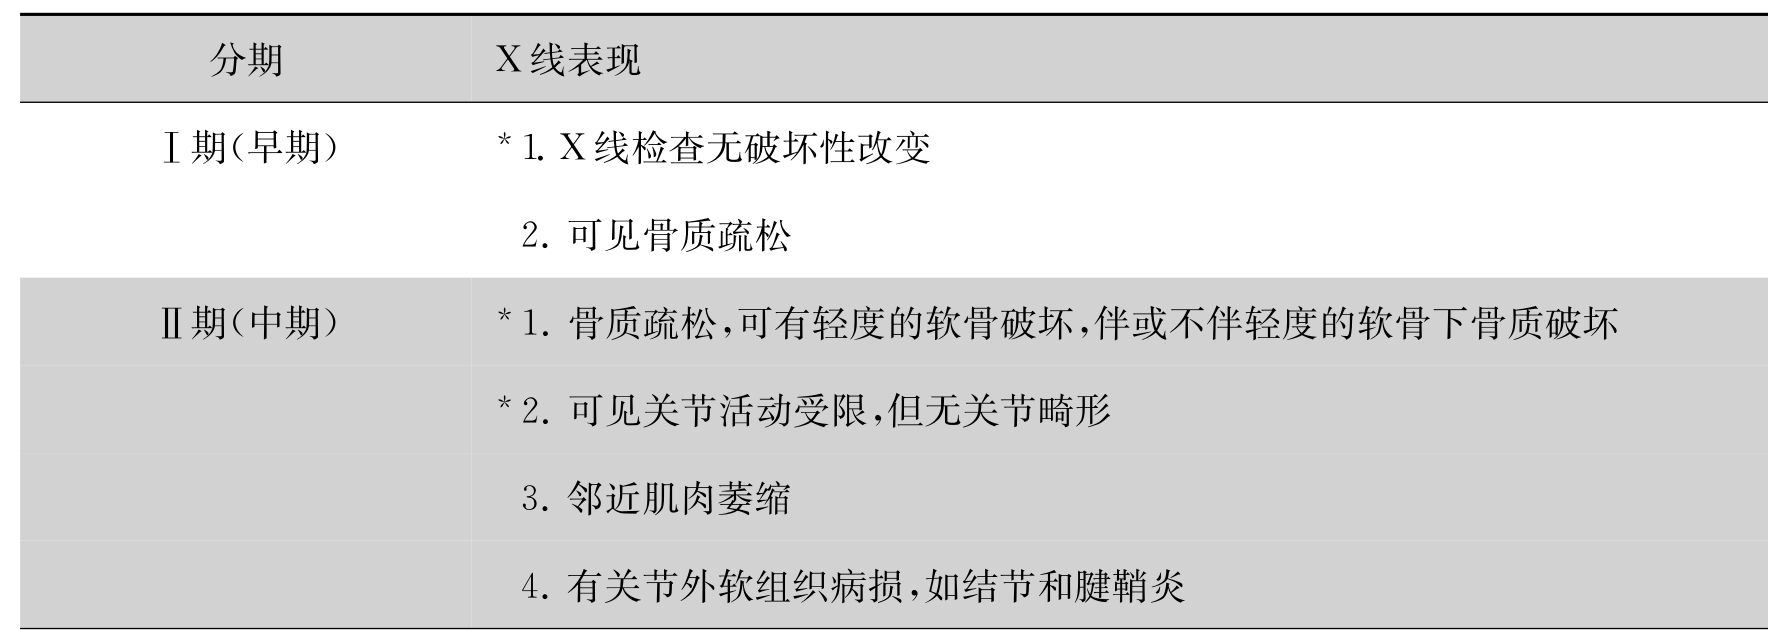
\includegraphics[width=\textwidth,height=\textheight,keepaspectratio]{./images/Image00257.jpg}\\
 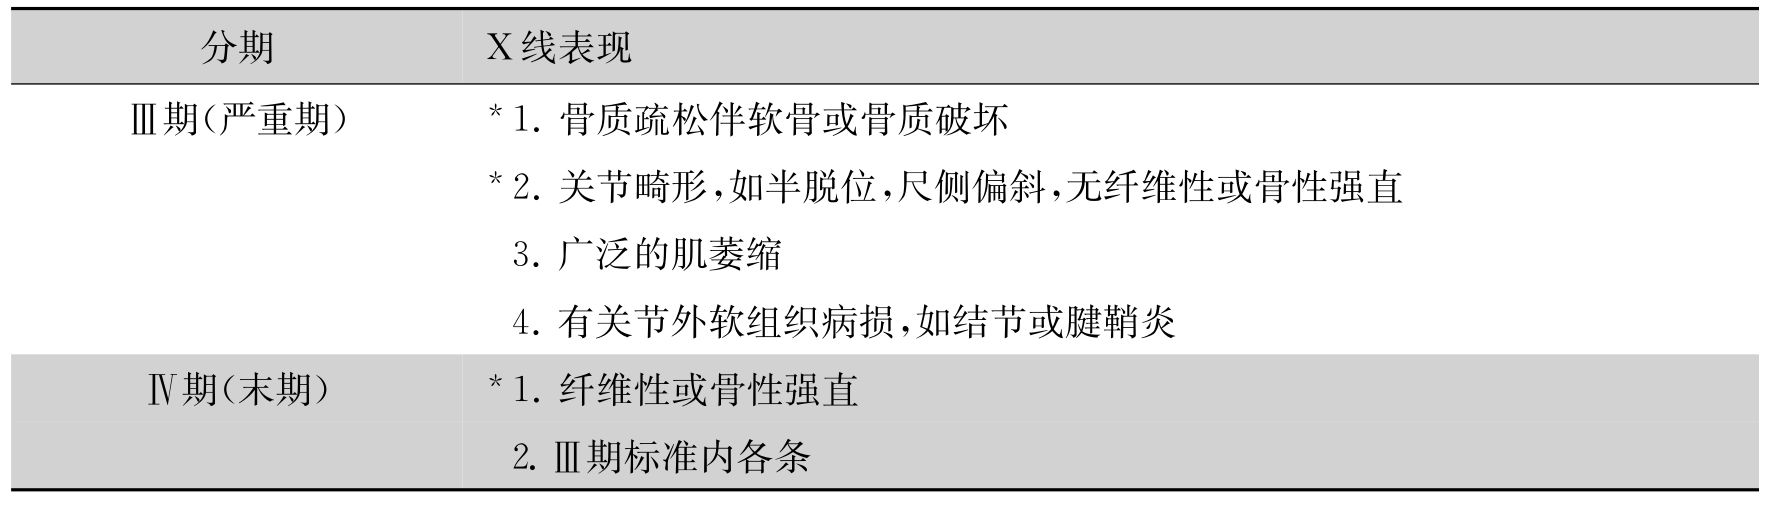
\includegraphics[width=\textwidth,height=\textheight,keepaspectratio]{./images/Image00258.jpg}
 \end{longtable}

类风湿关节炎的诊断,典型病例按美国风湿病学会1987年修订的类风湿关节炎的分类标准(表\ref{tab43-3}),而对于早期及不典型的较难诊断。少数不典型的类风湿关节炎在早期仅侵犯单关节,容易导致诊断的延误,此时需要与感染性关节炎或血清阴性脊柱关节病相鉴别。密切追踪观察是最终确诊的关键。

\begin{table}[htbp]
\centering
\caption{美国风湿病学会1987年修订的类风湿关节炎的分类标准}
\label{tab43-3}
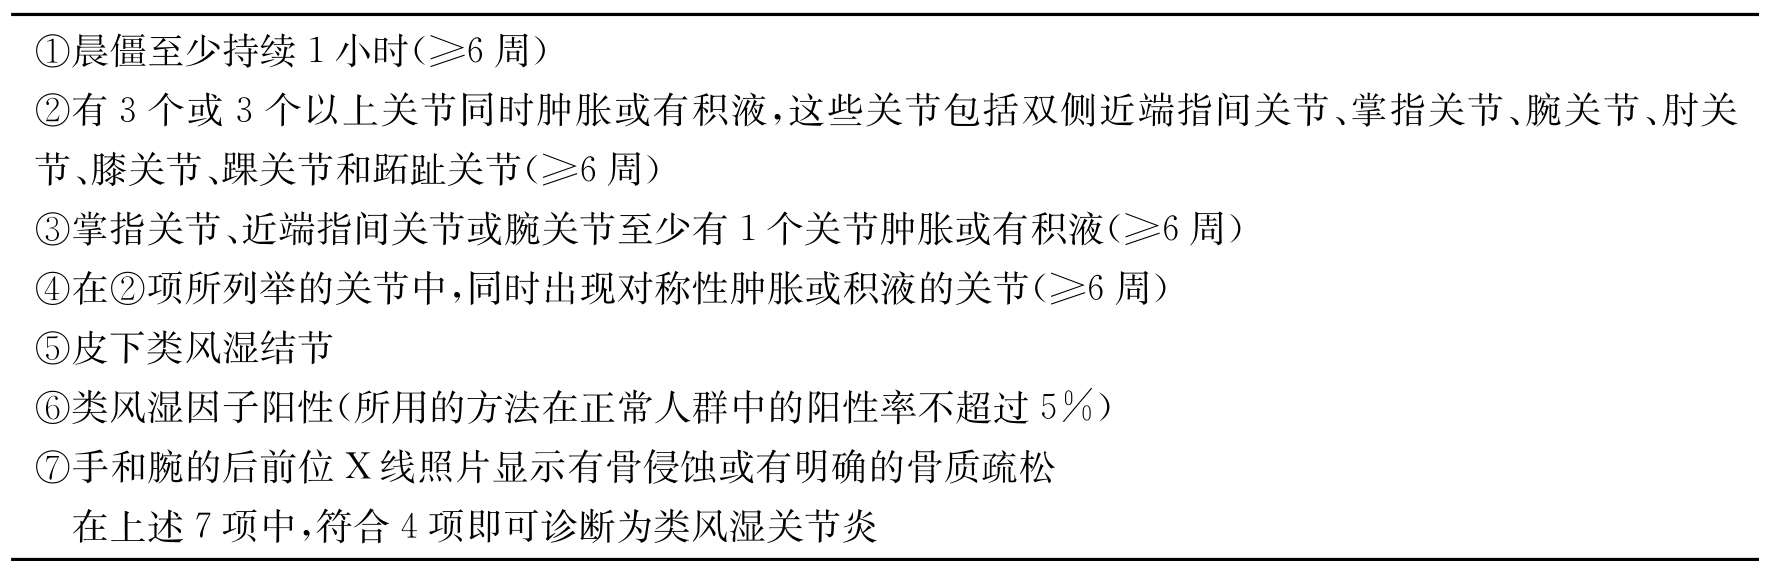
\includegraphics[width=5.89583in,height=1.89583in]{./images/Image00259.jpg}
\end{table}

2010年EULAR/ACR提出新的RA分类标准和评分系统,即:至少有一个关节的滑膜炎临床表现(肿胀);滑膜炎不能用其他疾病解释,并有典型的放射学RA骨破坏的改变,可诊断为RA。另外,该标准对关节受累情况、血清学指标、滑膜炎持续时间、急性期反应物4个部分进行评分,总得分6分以上也可确诊类风湿关节炎(表\ref{tab43-4})。

\begin{longtable}{c}
 \caption{EULAR/ACR 2010年RA分类标准和评分系统}
 \label{tab43-4}
 \endfirsthead
 \caption[]{EULAR/ACR 2010年RA分类标准和评分系统}
 \endhead
 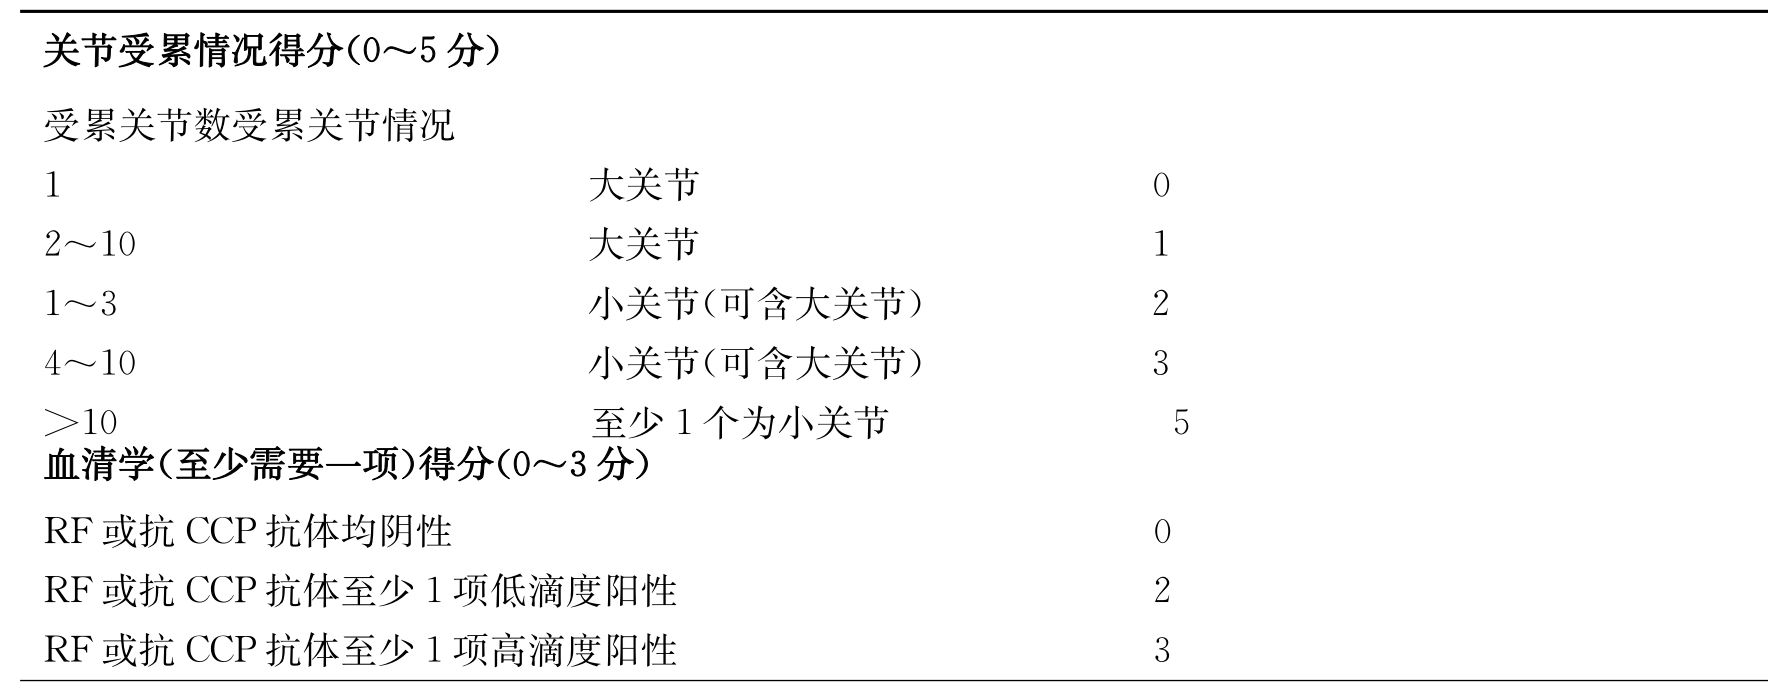
\includegraphics[width=\textwidth,height=\textheight,keepaspectratio]{./images/Image00260.jpg}\\
 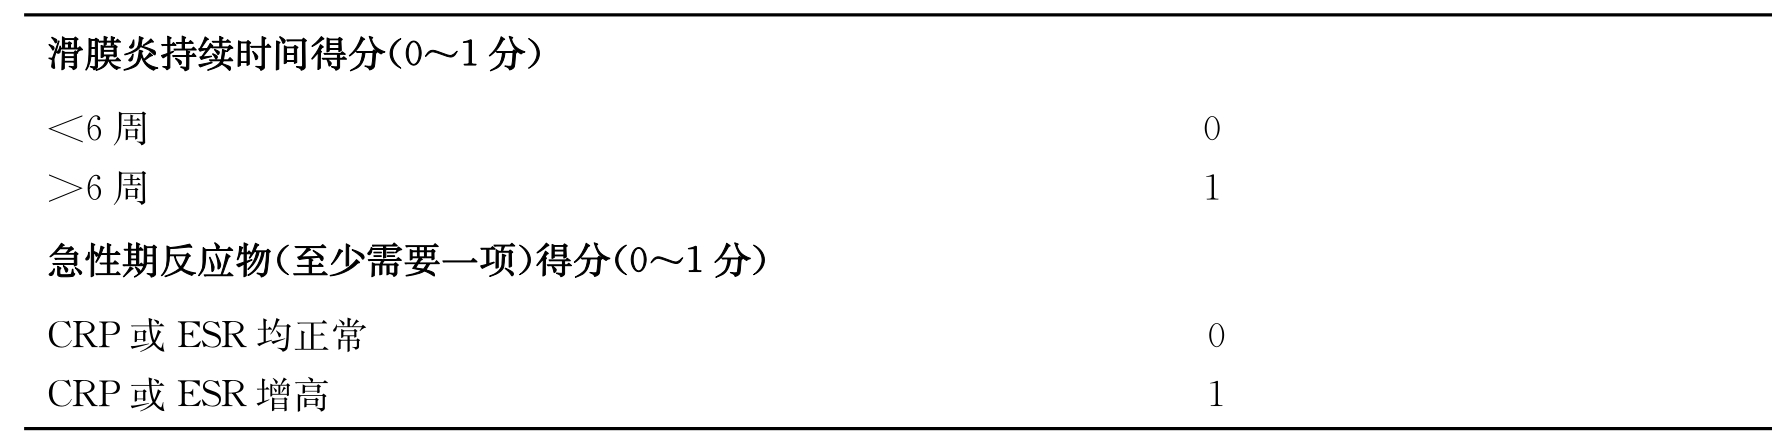
\includegraphics[width=\textwidth,height=\textheight,keepaspectratio]{./images/Image00261.jpg}
 \end{longtable}

类风湿关节炎需要与骨关节炎相鉴别,尤其是累及手指为主的增殖性关节炎,容易被误诊为类风湿关节炎(表\ref{tab43-5})。

\begin{table}[htbp]
\centering
\caption{类风湿关节炎与骨性关节炎的鉴别}
\label{tab43-5}
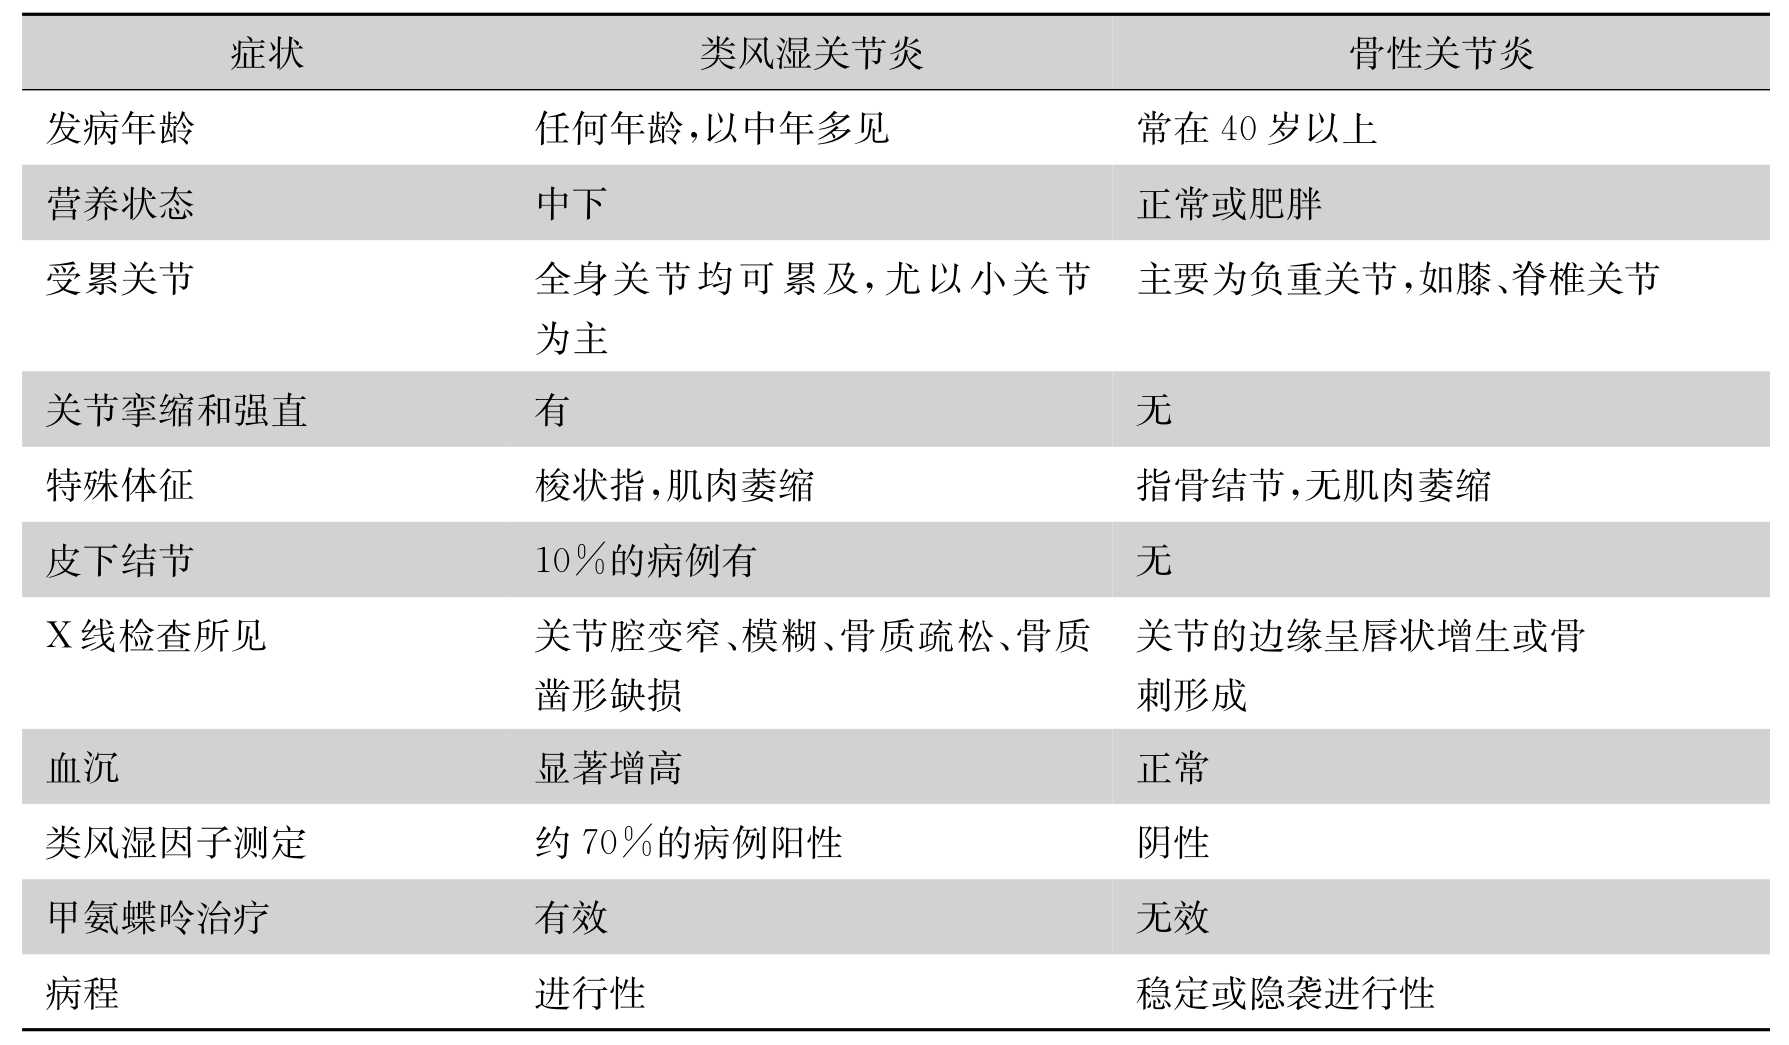
\includegraphics[width=5.95833in,height=3.47917in]{./images/Image00262.jpg}
\end{table}

本病尚需与结核性关节炎相区别。本病常侵犯多个小关节,而结核性关节炎几乎为单个关节病变,X线检查对鉴别帮助较大。疑难病例做关节腔抽出液动物接种与结核菌培养,可有助于鉴别诊断。

在临床上,类风湿关节炎可出现两种特殊的类型:

1.幼年型类风湿关节炎
幼年型类风湿关节炎又分为三种类型:全身型、多关节炎型和寡关节炎型。

幼年型全身型类风湿关节炎又称Still病,与成年人常见的类风湿关节炎不同,患儿往往以发热为突出表现。有时发生在关节炎出现之前数周或数月,也可以只在起病初期出现短暂的关节炎。多伴有多样化的非特异性皮疹,常见者为多形性红斑;皮下小结罕见。葡萄膜炎常见,可引起失明。可出现心包炎或心肌炎,但心瓣膜损害较少见。也常伴有肝、脾、淋巴结肿大。

幼年型类风湿关节炎的多关节炎型,在临床上与成年人的类风湿关节炎比较相似。也多以对称性多关节炎为突出表现。不过成年人的类风湿关节炎甚少累及远端指间关节,而幼年型类风湿关节炎有不少累及远端指间关节。

幼年型类风湿关节炎的寡关节炎型,多不对称地累及下肢大关节。这种患者须注意是否为以外周关节炎为首发表现的幼年型强直性脊柱炎,需要在随访中注意脊柱的症状。必要时行骶髂关节的放射学检查和血液HLA-B27检查。

2.Felty综合征
此综合征常发生于45~60岁,主要表现是类风湿关节炎伴发粒细胞减少、脾与淋巴结肿大,常有贫血。关节表现与典型的类风湿关节炎难以鉴别,其严重性可与血液学改变的严重程度不一致。血液学改变与脾功能亢进有关。类风湿性因子检查常为阳性,滴度常很高。脾切除后血象常恢复正常,但对关节炎的病程无恒定影响。

\subsubsection{(二)血清阴性脊柱关节病}

血清阴性脊柱关节病又称脊柱关节病,是指以中轴、外周关节以及关节周围组织慢性进展性炎症为主要表现的一组疾病。强直性脊柱炎是脊柱关节病的原形,除此之外,这类疾病还包括肠病性关节炎、银屑病关节炎、反应性关节炎、莱特尔综合征、未分化脊柱关节病等。

\paragraph{1.强直性脊柱炎}

强直性脊柱炎好发于青少年,男性明显多于女性。而且男性的病情往往较重,致残率高;而女性的病情往往较轻,致残率低。多数患者缓慢起病,以腰酸痛不适为主诉,或以腰骶部、臀部、颈部、肩背部疼痛为主。

腰骶部疼痛是患者最早和最常见的主诉,初时患者于晨间感腰骶椎关节僵硬、运动不灵、弯腰穿鞋困难,渐出现疼痛,继而病变向上发展累及胸椎与颈椎,出现胸背疼痛、气促,头部前后左右转动受限,脊柱可完全强直、僵硬。此类患者均有特殊的体征,表现为颈项前倾、胸段脊柱后凸(驼背),腰段脊柱失去正常的生理弯度而变平,躯干在髋关节处屈曲,前弯呈弓形。患者的全身症状如消瘦、乏力显著。

部分患者尤其是少年儿童的强直性脊柱炎,常常以下肢大关节肿痛为首发症状,因而造成误诊,值得临床注意,对于未能满足强直性脊柱炎的诊断者,需要注意跟踪随访,以便及早获得正确诊断。

本病的外周关节病变,以膝、髋、踝和肩关节居多,肘、手和足小关节偶见受累。非对称性、少数关节或单关节,以及下肢大关节的关节炎为本病外周关节炎的特征。患者除髋关节外,膝和其他关节的关节炎或关节痛多为暂时性,极少或几乎不引起关节破坏和残疾。髋关节受累占38\%~66\%,表现为局部疼痛,活动受限,屈曲挛缩及关节强直,其中大多数为双侧,而且94\%的髋部症状起于发病后头5年内。发病年龄小,及以外周关节起病者易发生髋关节病变。

实验室检查患者大多数有中度或高度血沉加快,C反应蛋白增高,球蛋白增高可导致A/G比值下降。虽然强直性脊柱炎患者HLA-B27阳性率达90\%左右,但无诊断特异性,因为也有5\%左右的正常人HLA-B27阳性。HLA-B27阴性患者只要临床表现和影像学检查符合诊断标准,也不能排除强直性脊柱炎。

由于强直性脊柱炎主要累及脊柱和下肢大关节,而早期的放射学改变往往报告骨质增生,在临床上需要与脊柱的骨性关节炎相鉴别。晨僵现象是其中最具有鉴别诊断意义的症状之一。有明显晨僵者,多考虑强直性脊柱炎。

强直性脊柱炎的基本病理改变是“肌腱-骨附着点”炎症。因此,患者往往表现出关节周围疼痛或肿痛,如足跟肿痛、膝关节下方相当于“足三里”附近的部位肿痛、肩胛骨疼痛、胸肋骨疼痛、髂骨或耻骨疼痛等等。

按目前诊断强直性脊柱炎的通用标准,骶髂关节损害的放射学改变是诊断该病的必备条件。所以对于临床上疑诊强直性脊柱炎的患者,有必要作骶髂关节的放射学检查,在此CT和MRI显像明显较X线平片清晰,更有利于早期诊断。但是,从骶髂关节损害至出现放射学改变,通常需要1~2年以上的时间,所以目前诊断强直性脊柱炎的标准无法对患者进行早期诊断。近年曾庆馀等报道,对临床上高度考虑强直性脊柱炎的诊断而缺乏骶髂关节损害的放射学证据者,行“CT引导下骶髂关节穿刺活检”,通过病理确定骶髂关节炎,有利于更早期诊断强直性脊柱炎。

髋关节损害是强直性脊柱炎致残的重要指征,所以对诊断或怀疑强直性脊柱炎的患者,应注意髋关节的症状,必要时作髋关节的磁共振检查。强直性脊柱炎自起病到脊柱强直是一个缓慢的过程,轻者可能一辈子不会出现脊柱强直,重者也需要5~8年才出现,多数患者在起病十几至二十年以上出现脊柱强直。多数患者开始时是炎症和肌腱因素导致的脊柱和关节活动受限,此时积极的抗炎和诱导缓解治疗以及康复性的功能锻炼,可以恢复功能,阻止或延缓病变发展为骨性强直。

强直性脊柱炎(AS)与类风湿关节炎(RA)有许多共同点,如:①两者均是自身免疫介导的,以侵犯关节为主的慢性、进行性、侵蚀性、致残性风湿性疾病;②均有明显的夜间疼痛加重和晨僵现象;③在疾病活动期均可有血沉、C反应蛋白增高;④非甾体抗炎药和激素有控制症状的良好疗效,但不宜依靠激素来治疗这两个病,而需要早期使用慢作用药,以缓解病情或控制病情的进展。因此过去曾经被认为是一个病的不同类型,当时强直性脊柱炎被称为是类风湿关节炎的中央型。20世纪60年代才确定这是两个不同的疾病,因此废弃“类风湿关节炎中央型”这一提法。强直性脊柱炎与类风湿关节炎的鉴别见表\ref{tab43-6}。

\begin{table}[htbp]
\centering
\caption{强直性脊柱炎与类风湿关节炎的鉴别表}
\label{tab43-6}
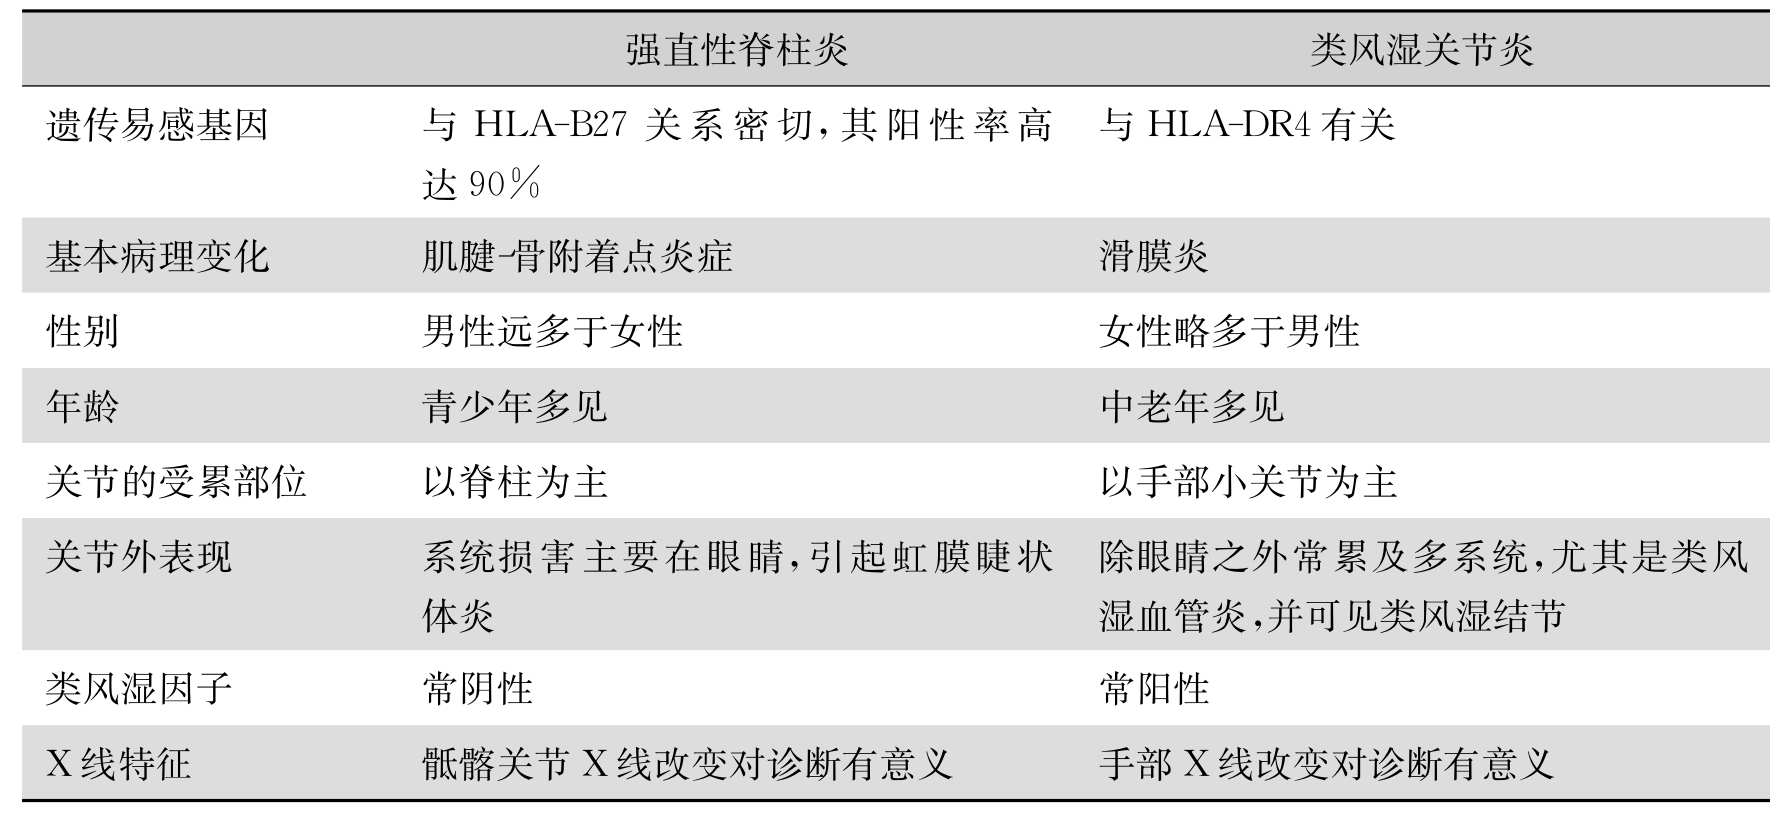
\includegraphics[width=5.9375in,height=2.70833in]{./images/Image00263.jpg}
\end{table}

\paragraph{2.其他血清阴性脊柱关节病}

除强直性脊柱炎外,血清阴性脊柱关节病还包括肠病性关节炎、银屑病关节炎、莱特尔综合征、未分化的脊柱关节病等,详见下文。

\subsubsection{(三)系统性红斑狼疮}

本病以年轻女性多见,关节症状见于90\%以上的患者,不仅在本病的任何阶段可见到,而且可以是最早期的症状,临床上可以表现为持续的关节疼痛,也可表现为急性或亚急性游走性多关节炎,容易被误诊为风湿热。受累关节呈不同程度的红、肿、热、痛,一般不出现关节畸形。如果出现侵蚀性关节损害,须注意重叠综合征(如红斑狼疮与类风湿关节炎重叠)。

如生育年龄女性不明原因出现发热、关节痛、血沉增快,需要考虑红斑狼疮的可能。如果伴有颜面部皮疹或多系统器官的损害,如肾脏损害、心脏损害、肝大、多浆膜腔渗出性炎症、白细胞减少以及雷诺现象等,更需要警惕系统性红斑狼疮。

抗核抗体必须作为关节炎尤其是生育年龄女性不明原因关节炎的常规检查项目,以免遗漏诊断。抗核抗体增高提示抗核抗体相关的结缔组织病,不能够确定是哪一个结缔组织病,需要进一步检查抗ds-DNA抗体和可溶解抗原系列的抗体(又称ENA系列抗体),如果抗ds-DNA抗体、抗Sm抗体阳性,则对系统性红斑狼疮的诊断有重要意义。美国风湿病学会2009年系统性红斑狼疮的诊断标准:

临床标准:①急性或亚急性皮肤狼疮表现;②慢性皮肤狼疮表现;③口腔或鼻咽部溃疡;④非瘢痕性秃发;⑤炎性滑膜炎,可观察到2个或更多的外周关节有肿胀或压痛,伴晨僵;⑥浆膜炎;⑦肾脏病变:尿蛋白>0.5g/d或出现红细胞管型;⑧神经病变:癫痫发作或精神病,多发性单神经炎,脊髓炎,外周或颅神经病变,脑炎;⑨溶血性贫血;⑩白细胞减少(至少1次细胞计数<4.0×10\textsuperscript{9}
/L)或淋巴细胞减少(至少1次细胞计数<1.0×10\textsuperscript{9}
/L),血小板减少症(至少1次细胞计数<100×10\textsuperscript{9} /L)。

免疫学标准:①ANA滴度高于实验室参考标准;②抗dsDNA抗体滴度高于实验室参考标准(ELISA法测需有2次高于该参考标准);③抗Sm抗体阳性;④抗磷脂抗体:狼疮抗凝物阳性/梅毒血清学试验假阳性/抗心磷脂抗体是正常水平2倍以上或抗β2GPI中滴度以上升高;⑤补体减低:C3、C4、CH50;⑥无溶血性贫血但Coombs试验阳性。

确诊条件:①肾脏病理证实为狼疮肾炎并伴ANA或抗dsDNA阳性;②以上临床及免疫指标中有4条以上符合(至少包含1项临床指标和1项免疫学指标)。该标准敏感性94\%,特异性92\%。

\subsubsection{(四)结节性多动脉炎}

约半数患者有关节痛,少数有明显的关节炎改变。约1/3患者骨骼肌血管受累而产生恒定的肌痛,以腓肠肌痛多见。疾病早期常可有下肢关节受累,表现为非对称性、非破坏性关节炎,在早期病例约占20\%,随病情发展这一比例可逐渐增高。结节性多动脉炎的关节炎特点是非对称的,非致畸性的间断发作,主要影响下肢大关节。患者经常出现与外周神经病变、肌肉关节受累、皮肤和胃肠道受累相关的疼痛。尽管有比较严重的肌痛,但肌酸激酶通常正常。受累关节的滑液检查无诊断意义,仅仅提示轻微的炎症。

\subsubsection{(五)硬皮病}

硬皮病又称为进行性系统性硬化症。主要侵犯皮肤,可伴有内脏(消化系统、呼吸系统和心血管系统)损害。除局限性硬皮病外,多数患者自手足开始起病。部分患者由轻度雷诺现象开始,缓慢加重,并出现关节疼痛。更多的患者起病时手部包括手指和手背肿胀、僵硬。晨僵明显,导致晨起时握拳困难。由于初期没有皮肤硬化的表现,容易被误认为是类风湿关节炎。其区别在于硬皮病的手指呈均匀性肿胀,手背明显肿起,并且多伴有雷诺现象。进一步发展手指皮肤开始变硬,出现腊肠样改变,几个月或十几个月后水肿消退、皮肤绷紧,最后皮肤萎缩,指端骨质吸收,指、趾、腕、肘等关节固定于屈位,呈蜡样手。

60\%~80\%系统性硬皮病(SSc)病例出现关节和肌肉的病变。系统性硬化早期常出现全身关节疼痛和晨僵。硬皮病的皮肤病变早期最常侵犯双手,表现为双手指肿胀、运动障碍,虽然真正的病变部位不是在关节,但因手指周围软组织硬化,引起肌腱挛缩而致手指屈曲畸形,可误诊为类风湿关节炎。病变由远端逐渐向近端发展,先以皮肤色素加深,后出现点状和斑片状色素脱落,形成“象牙白”的色素缺损,缺乏经验的医生会误诊其为“白癜风”。随着病情发展,本病的诊断并不困难,广泛的皮肤硬化、皮肤有蜡样光泽、面部表情固定似假面样、张口困难、吞咽障碍,以及肺间质纤维化等,均支持硬皮病的诊断。

\subsubsection{(六)皮肌炎}

在结缔组织病中,皮肌炎很少引起关节损害。只有少数患者出现关节痛以及关节周围肌腱、软组织疼痛。

\subsubsection{(七)混合性结缔组织病}

混合性结缔组织病(MCTD)是一种结缔组织病,其临床特征是具有类似于红斑狼疮、硬皮病、皮肌炎等的临床表现,其血清学特征是抗核抗体增高,抗ul-RNP抗体阳性,而抗ds-DNA和抗Sm抗体阴性。患者多有雷诺现象、关节疼痛和晨僵现象。几乎所有的MCTD患者都有比系统性红斑狼疮更常见、更严重的关节痛和关节僵硬。60\%的患者最终发展为显著的关节炎,通常伴有类风湿关节炎常见的关节变形,如尺侧偏斜、天鹅颈畸形和纽扣花畸形。少数患者可出现肋骨侵蚀性改变和屈肌腱鞘炎。

混合性结缔组织病与重叠综合征是两个不同的概念。前者是一个独立的疾病,后者是两个或以上的结缔组织病同时并存,重叠在一个患者身上。

\subsubsection{(八)干燥综合征}

干燥综合征是以累及外分泌腺为主的结缔组织病。绝大多数患者伴有关节肿痛,部分出现与类风湿关节炎一样的侵蚀性关节炎,后期少部分也可出现手指的尺侧偏斜、天鹅颈畸形、纽扣花畸形等。干燥综合征的突出表现是口干、眼干、阴道干。常常因为唾液腺分泌减少导致龋齿增多,严重者可在一年或几年之内全部牙齿龋溃,剩下牙根,称为“猖獗龋”。常见的系统损害包括间质性肺炎和肺间质纤维化、肾小管性酸中毒、胆汁淤滞性肝炎、假性淋巴瘤等等。实验室检查主要是抗核抗体增高、抗SSA和抗SSB抗体阳性,类风湿因子也常常阳性。关节病变较重的类风湿关节炎患者,尤其是中年女性,可合并继发性干燥综合征,但与原发性干燥综合征相比,少见严重的内脏损害。

\subsubsection{(九)白塞病}

40\%~60\%的患者表现为关节痛和外周关节炎。外周关节炎可以为单关节、少关节或多关节。主要影响下肢,以膝关节受累最为常见,其次为腕、踝、肘,表现为相对轻微的局限性、非对称性关节炎。大多表现为一过性关节痛,可反复发作并自限,偶尔可在X线上表现出关节骨面有凿样破坏,一般不引起关节破坏或畸形,极少为慢性过程。34\%的白塞病患者可出现骶髂关节炎,出现类似强直性脊柱炎的表现。受累关节表现出滑膜炎病变。滑膜的病理改变主要表现为滑膜浅层有中性粒细胞浸润和血管充血渗出等急性炎症性病变。滑膜细胞的增殖、淋巴细胞的浸润和淋巴滤泡的形成都很少见,说明其滑膜炎和类风湿关节炎不同。骶髂关节炎少见。

\subsubsection{(十)银屑病性关节炎}

银屑病又称牛皮癣,所以其关节炎又称牛皮癣性关节炎。银屑病是一种常见而容易复发的慢性皮肤病,皮肤病变好发于头皮及四肢伸侧,尤其肘、膝部位,呈散在或泛发分布,要特别注意隐藏部位的皮损如头发、会阴、臀、脐等,表现为丘疹或斑块,圆形或不规则形,表面有丰富的银白色鳞屑,去除鳞屑后为发亮的薄膜,除去薄膜可见点状出血(Auspitz征),该特征对银屑病具有诊断意义。存在银屑病是与其他炎性关节病的重要区别。

多数银屑病的关节炎发生在皮疹之后,银屑病数年之后才逐渐出现关节症状。也有一些患者的皮疹和关节炎同时出现,偶然也见先有关节炎,随访若干时间后才出现皮疹。多数银屑病性关节炎的关节症状,与皮肤损害的好转和恶化相平行。其临床特点为:指、趾小关节特别是远端指间关节常常受累,在远端指间关节受累的同时往往伴有指(趾)甲损害。指甲损害的特点是甲板增厚、凹陷或嵴形隆起。但有时肉眼观银屑病性关节炎的指甲损害与指甲癣不易区别,其特点之一是:银屑病性关节炎的指甲损害往往为对称性和多数指甲同时受累,不痒;而指甲癣多不对称,而且只累及少数1~2个指甲,有痒。甲屑找癣菌有助于鉴别诊断。

银屑病性关节炎可累及任何关节,包括中轴关节和各外周关节,导致关节疼痛、肿胀,最后可致关节强直与畸形。大、小关节均可受累。本病也属于血清阴性脊柱关节病的一种,但与强直性脊柱炎相比,除银屑病皮疹的区别之外,银屑病性关节炎更多地累及外周关节,而且常累及指、趾等小关节。银屑病性关节炎的HLA-B27阳性率远低于强直性脊柱炎,也低于肠病性关节炎。

有学者将银屑病性关节炎分为三种类型:①类似反应性关节炎伴附着点炎的单关节和寡关节炎型;②类似类风湿关节炎的对称性多关节炎型;③类似强直性脊柱炎的以中轴关节病变为主(脊柱炎、骶髂关节炎和髋关节炎),伴有或不伴有周围关节病变的脊柱病型。

由于银屑病性关节炎也常累及外周小关节,所以临床上需要与类风湿关节炎相鉴别。详见表\ref{tab43-7}。

\begin{table}[htbp]
\centering
\caption{银屑病性关节炎与类风湿关节炎的鉴别}
\label{tab43-7}
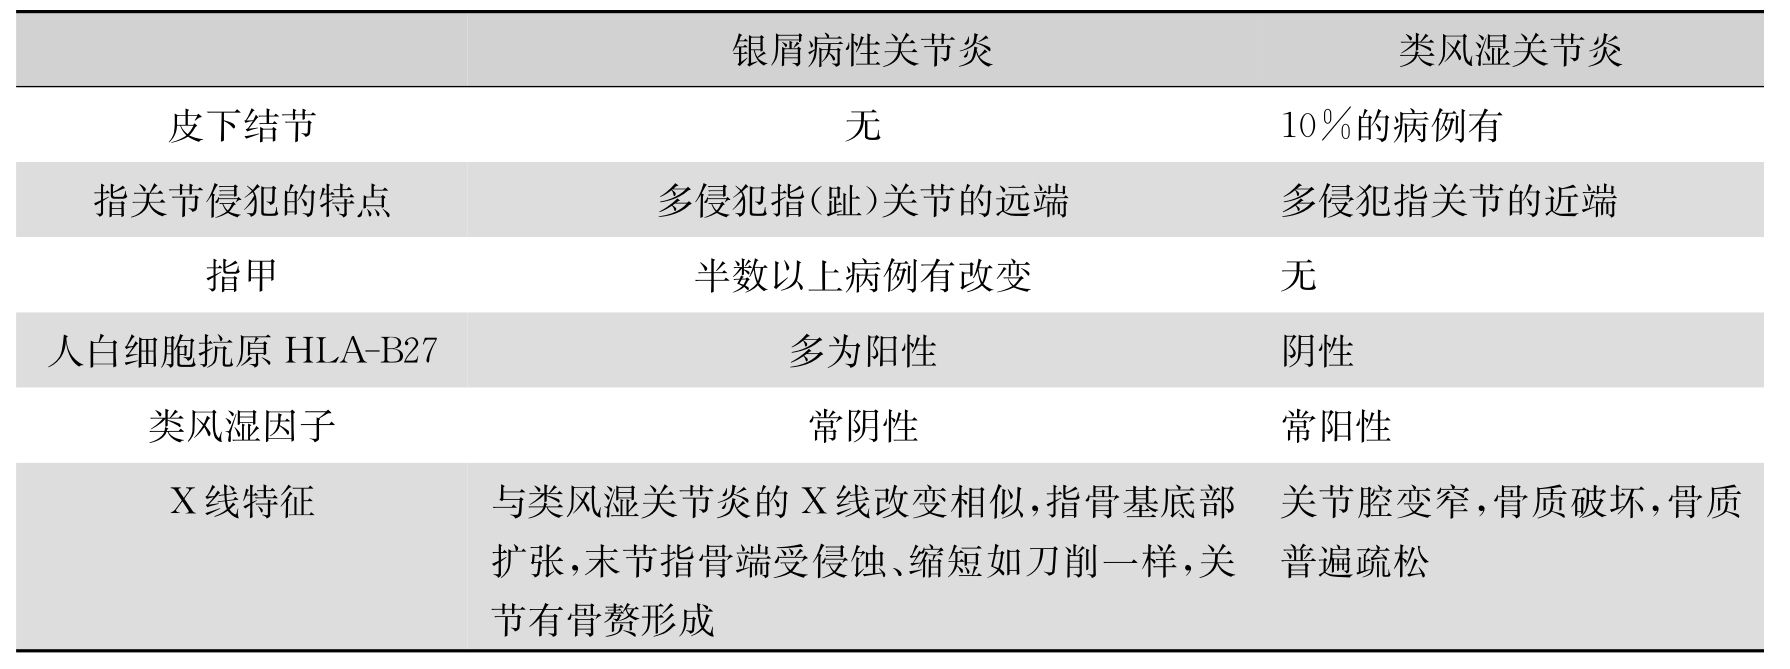
\includegraphics[width=5.95833in,height=2.21875in]{./images/Image00264.jpg}
\end{table}

\subsection{二、骨性关节病}

骨性关节病又称骨关节炎、增殖性关节炎、肥大性关节炎、变性性关节炎等,是一种以关节软骨变性、破坏及软骨下骨边缘骨赘形成为特征的慢性关节炎,在本质上并非炎症,更正确地说应属于退行性关节病。本病好发于老年人,发病率与年龄俱增,一般在40岁以后随着年龄的推移发病率逐渐增高。女性比男性更加明显。较常受累的关节为负重较大的关节,如膝、髋、脊椎等大关节。起病缓慢,呈潜隐性,早期往往无症状,或因其他原因进行X线检查而偶然发现病变的存在。其临床特点为罹患的关节酸痛、轻度僵硬,活动不灵;关节甚少肿胀,活动时出现摩擦音,不发生关节强直;触诊时可能发现关节边缘有增生的骨质凸起。患者无发热、贫血等全身症状,血沉正常,血清抗链球菌溶血素“O”滴度不增高,类风湿因子试验阴性。

骨关节炎虽有X线改变,但不一定有疼痛或关节功能障碍。无症状骨关节炎的发病率比有症状者更高。

部分骨关节炎对天气变化敏感,在天气变化前夕出现关节症状突然加重。多数骨关节炎患者有关节怕冷,在寒冷的环境中关节疼痛加重。

膝关节受累在临床上最为常见。最早期的症状是上、下楼或爬山时出现膝关节疼痛,进一步发展则行走时疼痛。严重病例可出现膝内翻或膝外翻畸形。

颈椎受累比较常见。可有椎体、椎间盘以及后突关节的增生和骨赘,引起局部疼痛和僵硬感,压迫局部血管和神经时可出现相应的放射痛和神经症状。颈椎受累压迫椎-基底动脉,引起脑供血不足的症状。腰椎骨质增生导致椎管狭窄时可出现间歇性跛行以及马尾综合征。

一种特殊类型的骨关节炎称为结节性骨关节炎,主要不是累及负重关节,而是累及手指小关节。以远端指间关节受累最为常见,表现为关节伸侧面的两侧骨性膨大,称Heberden结节。而近端指间关节伸侧出现者则称为Bouchard结节。可伴有结节局部的轻度红肿、疼痛和压痛。第一腕掌关节受累后,其基底部的骨质增生可出现方形手畸形,而手指关节增生及侧向半脱位可致蛇样畸形。这种类型的骨关节炎多见于50岁以上的女性,据报道女性发病约10倍于男性,多有家族性。其发生十分缓慢而隐袭,可以没有疼痛症状,但多有僵硬感和握力下降,许多患者主诉有晨僵现象。拇指的结节性骨关节炎多有疼痛,其他手指的结节性骨关节炎在结节长出来期间多有疼痛,之后多只是感觉僵硬,而无明显疼痛。这种类型的骨关节炎需要与类风湿关节炎鉴别,最关键的鉴别要点是远端指间关节是否受累。还有类风湿关节炎指间关节的滑膜炎性肿胀与结节性骨关节炎的骨赘性结节,在检查时手感是不一样的。所以,只要对这两个病有所认识,鉴别并不困难。

X线检查对增殖性关节炎的诊断有重要意义。早期在X线摄片上,已可见到明显的骨质增生、关节边缘唇状改变或(及)骨刺形成。晚期发生关节腔变窄,软骨下骨质硬化,周围韧带钙化。

骨关节炎一般不伴关节红肿,没有晨僵现象。但出现继发滑膜炎时,可以表现为红、肿、热、痛,也可以有短暂晨僵,晨僵时间多不超过半小时。出现继发滑膜炎的骨关节炎,需要与类风湿关节炎鉴别。

\subsection{三、代谢障碍性关节病}

\subsubsection{(一)慢性痛风性关节炎}

慢性痛风性关节炎是由于关节软骨及关节囊内积累尿酸盐所致。为病程迁延多年、持续高尿酸血症所引起,痛风石形成或关节症状持续不能缓解是此期的临床特点。急性痛风性关节炎开始时多累及单个关节,继而累及多个关节,经反复发作后逐渐发生关节变性,在关节附近软组织中出现痛风石(痛风结节)。痛风石最常见于耳壳和指(趾)关节,并继续增大,可向皮肤穿破,排出白色的尿酸盐结晶,肉眼观似石灰,显微镜下见尿酸盐结晶。痛风石破溃物中发现尿酸盐结晶,对本病的诊断有决定性意义。

患者常并发痛风性肾病和尿酸性肾结石。痛风性肾病主要表现为肾间质损害,开始时表现为夜尿增多,后期可导致肾衰竭。尿酸性肾结石有时出现肾绞痛,也可出现梗阻性肾病。痛风性肾病和尿酸性肾结石均有可能导致肾性高血压,持续的高血压对肾功能本身又是负面影响。所以慢性痛风的患者需要注意肾脏的问题。

痛风与痛风性关节炎的主要诊断根据:

1.典型的急性或慢性痛风性关节炎发作,尤其是痛风石的出现。

2.血中尿酸增高,男>428μmol/L,女>357μmol/L。

3.X线检查可见关节面附近的骨骺部因骨组织被尿酸所替代而出现圆形缺损。

4.痛风结节溃破处的分泌物镜检或活检发现针状尿酸盐结晶。

5.诊断性治疗 秋水仙碱对痛风性关节炎有特殊疗效,而对其他原因的关节炎无效。

痛风按照病因分为原发性和继发性两大类。原发性痛风有一定的家族遗传性,约10\%~20\%的患者有阳性家族史。除1\%左右的原发性痛风由先天性酶缺陷引起外,绝大多数发病病因不明。原发性痛风在成年男性的各个年龄组均可出现,而女性主要见于绝经期以后。过去认为痛风主要与家族遗传有关,现在认为饮食结构与痛风的关系更密切。继发性痛风可见于真性红细胞增多症、白血病、恶性肿瘤(特别是在化疗之后),慢性肾脏病、肾铅中毒、器官移植后运用环孢素等药物也可导致高尿酸血症和痛风。按照痛风的自然病程可分为急性期、间歇期、慢性期。

\subsubsection{(二)假性痛风}

痛风需与假性痛风相鉴别。假性痛风是由焦磷酸钙沉积于关节软骨引起,急性发作时,表现与痛风酷似,但有下述特点:①老年人多见;②病变主要侵犯膝、肩、髋等大关节;③X线摄片见关节间隙变窄和软骨钙化灶呈密点状或线状,无骨质破坏改变;④血清尿酸含量往往正常;⑤滑液中可查见焦磷酸钙单斜或三斜晶体;⑥秋水仙碱治疗效果较差。曾报告有家族性病例。诊断主要根据病史、X线摄片检查以及罹患关节的滑液检查。关节滑液中在急性发作期有大量中性粒细胞,焦磷酸钙二水合物结晶常发现于细胞外或中性粒细胞内;在慢性病例中这些结晶较少见,如有发现,则最常位于中性粒细胞之内。本病国内仅见少数报告。

\subsubsection{(三)褐黄病}

褐黄病(ochronosis)是罕见的先天性疾病,主要临床表现是黑色尿,耳软骨呈蓝灰色,巩膜上可见黑斑和皮肤棕色色素沉着,病情进展时常于30~40岁左右出现慢性多发性关节病变。关节病变除色素沉着于软骨外,还伴有退行性变。关节炎症缓慢进展,首发症状多为下背部痛、僵硬、活动受限制以及正常的腰椎生理弯曲消失,数年之后可侵犯颈椎和整个脊椎,以致脊椎强直。X线特征是椎间盘钙化、椎间隙变窄以及椎体边缘有骨赘形成。与强直性脊柱炎不同的是骶髂关节并无融合,关节面正常,同时脊椎无竹节样改变。病情继续发展,邻近四肢的大关节如髋、膝和肩关节常受累,常见的症状为关节疼痛、僵硬,关节活动时有响音,运动受限。部分病例发生关节渗液,渗液中有黑酸尿存在。X线特征主要为退行性关节病变。此病一般极少侵犯手、足小关节,无全身症状,类风湿因子试验阴性,可与类风湿关节炎相区别。本病的诊断不难,患者尿静置后变为黑色,常提示黑酸尿的存在。

\subsection{四、慢性感染性关节炎}

\subsubsection{(一)结核性关节炎}

关节结核是全身性结核感染的局部表现,特别多发于儿童及青少年,常为慢性经过。病变最多发于支持体重而活动较多的关节,常侵犯脊柱,髋、膝关节,多为单关节炎。关节疼痛、肿胀,晚期关节功能障碍、畸形和强直。脊柱结核常累及腰椎、胸椎,表现为腰痛、背痛、神经根痛,患椎周围肌肉痉挛,局部叩痛明显,脊柱活动受限和后凸畸形,可有寒性脓肿及窦道形成。病情严重者合并偏瘫。

本病的主要诊断根据:①有结核病史,并出现消瘦、微热、盗汗、疲乏等全身中毒症状;②罹患关节疼痛(负重和活动时加重),常在睡梦中痛醒,早期即有关节明显肿胀及肌肉萎缩,后期关节畸形与功能障碍,寒性脓肿及瘘管形成为本病的特点;③活动期血沉升高;④X线检查发现关节腔变窄、骨质局限性破坏,或在椎体周围显示脓肿阴影,对诊断帮助很大,由于X线征象比临床症状出现较晚,且为重要的诊断依据,一般需作正、侧位摄片,必要时作CT或MRI检查,以协助早期诊断;⑤关节腔抽出液检查:混浊,中性粒细胞增多,蛋白质含量高,20\%患者滑液涂片抗酸染色可找到结核杆菌,结核杆菌培养80\%为阳性;⑥滑膜活检可发现结核结节和干酪样变;⑦结核菌素试验对诊断也有重要的参考价值。

结核性关节炎的临床表现与X线征有时与类风湿关节炎难于区别。结核性关节炎较常侵犯单个大关节,而类风湿关节炎最常侵及多个中、小关节,为对称性多关节炎,晨僵明显,类风湿因子阳性,细菌学及病理学可予以鉴别。

早期的髋关节结核,有时与以髋关节为主要表现的血清阴性脊柱关节病难以鉴别。两者均有血沉和C反应蛋白增高,类风湿因子均阴性,两者均是夜间疼痛加重。鉴别方法:①HLA-B27在血清阴性脊柱关节病的阳性率为80\%~90\%,而在髋关节结核与普通人群一样只有5\%;②髋关节磁共振检查,周围软组织肿胀在髋关节结核比血清阴性脊柱关节病明显;③试验性抗结核治疗:三联抗结核治疗2~4周,症状减轻者提示髋关节结核;④试验性抗风湿治疗:短时间微小剂量激素,泼尼松10mg/d,疗程1~2周,对血清阴性脊柱关节病有止痛作用,而在髋关节结核的止痛作用不明显;⑤髋关节的关节镜检查对两者的鉴别诊断有重要意义,但如果是在病变的早期,尚未出现干酪样坏死,有时也会有不确定性的病理报告;⑥放射学检查的动态观察,在上述方法均难以作出准确的鉴别诊断时,放射学检查的动态追踪显得非常重要,一般要求每2~3个月作一次放射学检查,多数情况下髋关节结核在3个月左右可见有放射学改变,而血清阴性脊柱关节病一般需要6~12个月以上才可见有放射学改变。

脓肿形成时需与化脓性关节炎鉴别。化脓性关节炎起病急,关节红肿热痛及压痛明显。主要通过细菌学及病理学检查予以鉴别。

\subsubsection{(二)梅毒性关节炎}

梅毒性关节炎是因梅毒螺旋体侵入关节滑膜所引起,主要发生于二期或三期梅毒。

二期梅毒性关节炎好发于四肢大关节,依次为肩、肘、膝、髋、踝等关节,常为对称性及多发性,小关节较少累及。关节炎可在发疹前出现,其特点为罹患关节钝痛,疼痛甚轻微,无游走性,功能障碍轻微或缺如,皮肤无急性炎症,仅轻度肿胀。X线检查关节面软骨无损害。梅毒血清反应常呈强阳性。驱梅治疗的初期关节疼痛反而加剧,继续驱梅治疗后关节症状迅速消失。水杨酸制剂无疗效。

三期梅毒的关节损害发生于感染后3~5年,或迟至10~30年。此型关节炎罕见,为梅毒肉芽肿由邻近组织侵入关节所产生。病变好发于膝关节,但胸锁、胸肋及指关节也可罹患。受累关节微痛,常于夜间加剧,运动后痛减轻,关节腔内可有轻度渗出液,但表皮无红、肿、热表现。如骨端树胶肿向外穿破形成瘘管,需与结核性关节炎鉴别。患者的梅毒血清反应大多阳性,常并发皮肤、黏膜、心血管、神经系统及内脏的梅毒损害,易与结核性关节炎区别。

晚期关节梅毒也需与风湿热的关节炎和化脓性关节炎区别,可根据性病史、上述症状与体征、梅毒血清反应以及驱梅治疗的疗效等鉴别之。

\subsubsection{(三)Reiter综合征}

莱特尔综合征(Reiter综合征)由包涵体结膜炎衣原体感染所引起。此综合征具有尿道炎、结膜炎与关节炎三联症。关节炎常常为非对称性,如果没有及时获得恰当的治疗,多演变为慢性、侵蚀性关节炎,部分病例最终出现关节畸形与功能障碍。莱特尔综合征是一种特殊类型的反应性关节炎,具备典型的急性关节炎、非淋球菌性尿道炎和结膜炎三联症者确诊并不困难,但由于各种表现可在不同时期出现,所以诊断有时需要数月时间。发展为慢性莱特尔综合征患者,其关节炎和(或)皮损的表现类似银屑病性关节炎、强直性脊柱炎和白塞病。

\subsubsection{(四)莱姆病}

莱姆(Lyme)病是一种蜱媒螺旋体感染、侵犯多系统的炎症性疾病。本病最初成批地集中发生于美国康涅狄格州Lyme市的儿童,故因此而得名。典型的发生于夏季。特征性表现是游走性慢性红斑,可先有发热或伴同发热而出现。其他症状为乏力、头痛、颈硬、神经系统或(及)心脏病病征等,关节炎可在数周或数月之后出现。约50\%患者发生关节炎,关节表现为间断性关节肿胀和疼痛,主要累及大关节,以膝为多,其他为肩、肘、腕、髋、踝、颞颌及四肢小关节。以单关节或少数关节受累居多,少数病例多个关节受累,多为非对称性分布。关节症状持续数周、数月甚至数年,可发展为慢性病变。

1986年曾在黑龙江省海林县发现一些病例,表现为慢性游走性红斑、慢性脑膜炎、面神经麻痹、多发性关节炎等,初步调查表明该地有Lyme病流行。

\subsection{五、血液病所致的关节病}

\subsubsection{(一)血友病性关节病}

血友病是一种缺乏抗血友病球蛋白的出血性疾病,仅发生于男性。患者常因轻微外伤或自发性四肢、肌肉、关节及内脏出血,尤其是关节内出血最常见。膝关节最常累及,踝、肘、髋关节次之。关节急性出血时患者突然体温升高,关节剧痛、迅速肿胀、不能活动,待血液吸收后关节外形及功能均恢复正常。如关节反复出血,吸收不全,血肿机化,滑膜及关节囊增厚;血肿压迫还可引起骨与软骨营养不良、坏死与吸收,晚期逐渐形成关节挛缩,致使关节呈屈曲性畸形。

X线有比较特征性表现,对诊断有一定价值,早期出血阶段关节囊胀大,关节间隙变宽,阴影的密度较大,比一般的滑膜炎明显。慢性骨关节病时,软骨面破坏,关节间隙狭窄,常见软骨下有囊样改变区,关节囊附着部骨质有腐蚀现象。年长者关节边缘有唇样增生。

本病颇易误诊,鉴别诊断上应与关节结核、类风湿关节炎、骨关节炎等鉴别;主要依靠既往有易出血的病史、血液学检查的凝血机制障碍表现,以及X线特征以鉴别。

\subsubsection{(二)其他血液病所致的关节病变}

白血病(尤以慢性型的急性变阶段)、骨髓纤维化、恶性淋巴瘤、多发性骨髓瘤等在病程中可发生骨、关节酸痛,有时可被误诊为“风湿病”。文献报道一例急性淋巴细胞白血病,因以左髋关节疼痛为主诉而误诊为左髋关节结核,经抗结核治疗无效,最后骨髓检查证实为白血病。

\subsection{六、神经源性关节病}

神经源性关节病是一种罕见的畸形性关节病,其主要病因为脊髓痨、脊髓空洞症等,此外为脊髓损伤、周围神经病变等。糖尿病引起本病者也有个案报告,主要发生于长期糖尿病而未适当治疗的患者。

本病好发于40岁以上的女性,由脊髓空洞症所致的多侵犯上肢关节,由脊髓痨所致的多累及膝、髋关节。脊椎关节罕见受累。临床上最特别的是关节始终不痛,甚至关节内发生骨折也不感觉疼痛,此外关节肿胀、无力、动摇、松弛(可向各个方向摇动的松弛关节),也与其他病因的关节病不同。

X线检查有助于此病的诊断,可见关节有明显的结构紊乱与破坏,常有骨赘生成,多并发脱位与病理性骨折。

\subsection{七、外伤性关节炎}

由于外伤或持续的慢性机械损伤,遗留关节疼痛与退行性病变者,称为外伤性关节炎。关节扭伤处理不当、关节骨折整复不良、膝关节半月板破裂治疗不及时,以及畸形所致关节负重不平衡(如膝内、外翻,脊柱侧弯,足部畸形)等,均可引起关节损伤。膝关节是全身关节中最易受伤的关节,其次为踝、肘、肩、髋等关节。踝关节损伤多见于足球、体操、篮球、滑雪和举重运动员以及舞蹈演员。其发病原因主要由于关节活动过度或关节软骨损伤所致,也与扭伤后过早参加练习有关。

下列几点有助于外伤性关节炎的诊断:①重体力劳动者或运动员,外伤前关节功能正常,症状发生于外伤或慢性劳损之后;②罹患的关节肿胀、压痛、运动障碍,尤以活动过多时出现疼痛;③骨关节X线检查常有阳性结果。根据上述情况,鉴别诊断一般不难。

\subsubsection{附:Hogga病}

本病是较少见而难以确诊的膝关节病变。病理基础为反复发生的慢性损伤引起的脂肪垫增生、炎症,和脂肪垫在胫股关节前方或髌股关节下方夹挤和撞击所致。关节镜下可作出诊断和满意的治疗。国内首次报道一组20例。

\subsection{八、其他原因}

\subsubsection{(一)大骨节病}

本病有一定的地域性,好发于7~18岁的青少年,无明显的性别差异,病因未明,主要病变在管状骨,表现为骨髓过早骨化、骨轴发育障碍、关节软骨破坏以及不规则的骨生成等。

膝、指、踝关节受累最多。起病缓慢,患者出现倦怠、四肢无力、关节运动不灵与关节疼痛。如出现手指关节对称性肿大、屈曲及背部隆起体征,则颇有助于早期诊断。晚期出现短指畸形、指关节增粗和摩擦音。膝关节受累时,由于双侧关节肿大、畸形和痉挛,致双膝外翻(“O”形腿)或双膝内翻(“X”形腿)。发病年龄较幼者,由于全身骨骼发育过早停止而形成侏儒。发病年龄越早,关节变形和侏儒越为明显,成人患者的症状一般较轻,常仅限于关节。血常规检查一般正常。患者血清钙与碱性磷酸酶升高,血清无机磷增高。

本病早期即可发现明显的X线改变,表现为掌指骨的骨骺线不完整,凹凸不平,呈波浪状或锯齿状,此病征对早期诊断很有意义。晚期骨端破坏、变形及肿大。罹患的关节腔变窄,关节面不整齐,骨质密度增高,并有骨唇突起。干骺和骨骺愈合,骨的长径短于正常。

如患者来自地方病区,呈慢性对称性关节增粗和身材矮小,并有短指畸形,则不难确定诊断。大骨节病需与类风湿关节炎鉴别。后者的发病年龄较晚,以青壮年多见,全身症状较明显,关节肿胀、畸形及骨性强直,常有梭形指,血沉加快,X线有特征性改变,无短指畸形。本病也需与呆小症区别,但患者的智力发育正常,也无呆小症的头大、脸宽、唇厚、舌大和流涎等特征。

\subsubsection{(二)慢性肺性肥大性骨关节病}

肥大性骨关节病是一种由于骨周围软组织增厚,广泛性骨膜新骨形成而导致的综合征。临床以杵状指(趾)、广泛性骨膜新骨形成和关节疼痛、积液为主要表现,分原发性和继发性两种。原发性肥大性骨关节病有家族史,为常染色体显性遗传,多于青春期发病,主要表现为杵状指(趾)、厚皮骨膜病,骨关节疼痛。继发性者以肺性肥大性骨关节病(PHO)最常见。

慢性肺性肥大性骨关节病的特点为多发性关节炎、骨膜炎与杵状指(趾)。国内报告大多数患者以类风湿关节炎的症状而就诊。膝、肘、腕、踝等关节常被累及。本病约90\%合并胸腔疾病,而80\%合并肺内疾病,其中2/3为支气管癌,1/5为良性肿瘤。少数合并心脏疾病和胸腔外疾病(如肝硬化、结肠炎)。有时也为特发性。临床上由于骨关节症状往往先出现,经过数月至数年才出现肺部症状,因此不少患者长期被误诊为类风湿关节炎等风湿性疾病。特别是骨关节病变多继发于周围型肺癌,而此型肺癌早期往往无呼吸道症状,故本病的发现对早期诊断肺癌有重要提示。

慢性肺性肥大性骨关节病的诊断根据是:①逐渐出现的杵状指(趾),四肢大关节(如膝、踝、腕)疼痛、肿胀与运动受限;②典型的X线征为长骨慢性进行性和对称性骨膜增生,如花边样或葱头样多层,此改变以胫、腓、尺、桡骨较常见;③肺部病灶(常见者为支气管癌)的存在。本病与类风湿关节炎的鉴别要点是杵状指与X线特殊改变(包括肺部肿瘤与长骨骨膜增生)。

原发性肥大性骨关节病亦称家族性厚皮性骨膜病,临床上罕见,国内仅有少数病例报告,与肺性肥大性骨关节病不同,后者的特点为:①无阳性家族史;②很少有皮肤病变;③关节疼痛常是唯一的症状;④原发病总是发现在肺、心、肝等脏器。

\subsubsection{(三)其他疾病所致的关节病变}

\paragraph{1.炎症性肠病}

炎症性肠病,包括慢性溃疡性结肠炎和克罗恩病的病程中,有部分并发周围关节和脊椎的炎症性病变,约20\%病例有外周关节炎,10\%~15\%患者有中轴关节炎。在消化科,这属于炎症性肠病的肠道外表现之一。而在风湿科,则称为肠病性关节炎,属于血清阴性脊柱关节病范围中的一个病。

有研究报告的79例有活动性溃疡性结肠炎的患者中,49例(62\%)有关节受累。受累的周围关节主要是大关节,特别是髋、踝和膝关节,非对称性。起病大多隐匿,呈轻微关节痛或僵硬感,也可出现红、肿、热、痛的急性关节炎症状,大多数患者同时有明显的肠道症状,可表现为阵发性肠绞痛、血便或腹泻等。但关节症状一般与肠道病变的严重程度并不平行。克罗恩病可出现杵状指,而骨膜炎罕见。大多数病例肠道症状先于关节表现或同时出现,但关节症状也可能先于肠道症状数年。

以脊椎炎为突出表现者,可有与强直性脊柱炎相似的临床表现,如腰背部钝痛或僵硬感,弯腰和伸展脊椎困难,也有明显的夜间疼痛加重和晨僵现象。肠病性关节炎的放射学也可显示骶髂关节损害,也与HLA-B27有一定的关系,有时肠病性关节炎与强直性脊柱炎没有明确的界限,因为同属于血清阴性脊柱关节病。区别在于前者同时有炎症性肠病,而后者没有。

以外周关节受累为主者,需与类风湿关节炎鉴别,主要区别点在于:肠病性关节炎的外周关节损害多为非对称性的;以大关节为主,少数侵犯手、足小关节者往往是不对称性的少数1、2个指(趾)关节;有明显的肿痛,容易变形;多伴有脊柱症状;类风湿因子试验阴性。

\paragraph{2.胆道感染}

胆道感染引起关节症状者也有报告,有的患者以发热、多发性关节肿痛与运动障碍就诊,颇似风湿性疾病。隐袭型胆道感染的患者无胆绞痛,而有关节症状时也可误诊为“风湿病”,但消化不良症状与胆囊压痛点压痛提示胆道感染的诊断,有怀疑者应作十二指肠引流术与胆囊造影检查。

\paragraph{3.潜水员减压病}

潜水员减压病最常引起骨关节病变,可见于造船、造桥、打捞和修建码头的潜水工作者。发病机制主要由于从高气压转至正常气压(减压)较快,以及机体内聚积过多的氮所引起。当潜水员潜水深度超过10cm(约增加1个大气压)时,氮气在组织内的溶解度增加一倍,因此,部分潜水员由于深度潜水后不遵守逐渐减压的常规而突然上升至水面时,组织内过多溶解的氮气就迅速游离成气泡,进入血液,造成血管的气栓,因气泡栓塞的部位不同而引起不同的临床表现。在皮肤引起瘙痒、出血;在中枢神经系统可致昏迷、瘫痪、失语、失明,甚至死亡;在肺部可引起呼吸困难、肺水肿等。最常见的是运动器官疾病,主要是营养骨膜下、骨、关节、肌腱、肌肉的血管气泡栓塞,引起骨内缺血性梗死,无菌性坏死,甚至破坏关节。最常见的临床表现是在四肢大关节出现突然剧痛,主要发生在关节周围及附近的肌肉、肌腱,使关节处于弯曲状态,伸直则痛增加,故称为“弯痛”,多呈刺痛、搏动痛或酸痛性质。轻者仅累及一个大关节,重者可多个关节甚至双侧四肢大关节同时发生弯痛。

潜水病持续的时间较长,可出现骨关节病变的异常X线征。主要在肱骨和股骨头部有骨骼缺血性坏死病变、骨质改变、骨骺线持续存在、骨骼内气泡样病变和骨关节炎病变。

本病的弯痛往往于工作后才突然发生,可误认为骨折或脱位,但患者有明确的职业病史,进入高压氧舱后疼痛马上减轻或消失,是诊断与鉴别诊断的主要依据。

\paragraph{4.骨、关节淀粉样变性}

淀粉样变性是少见的疾病,而骨、关节淀粉样变性更为少见,国内仅有个案报告。淀粉样变可分为原发和继发两类。原发性淀粉样变性是浆细胞病的一种,多侵犯血管壁﹑结缔组织﹑胃肠道平滑肌﹑末梢神经﹑心肌及肝﹑肾等实质器官﹐常引起胃肠出血及心肾衰竭而致死。继发性淀粉样变性较原发性为多见,继发于慢性病,如类风湿关节炎、结核病、慢性化脓性疾病等,多侵犯肝、脾、肾。

骨关节淀粉样变性多侵犯肩、肘、髋关节及关节附近的骨质。骨质有广泛性溶骨性破坏,主要在关节附近。罹患的关节肿胀,触之软而有弹性,肤色正常,皮肤温度正常,压痛不明显。

实验室检查可发现贫血与血浆蛋白减少。刚果红试验阳性(第1小时潴留量达90\%),但阴性不能除外本病。病理活检所见为变性的组织,标本放入卢戈碘液中则变成紫色。

\paragraph{5.复发性多软骨炎}

本病是一种病因未明的少见病。由于本病常首发于耳、鼻、咽喉及眼,不易被内科医师认识,常贻误诊断。该病可累及气道、外周关节和肋骨处的透明软骨,耳廓、鼻梁的弹性软骨,中轴关节的纤维软骨和存在于眼睛、心脏、血管、内耳等器官组织中的富含蛋白多糖的软骨共同基质也可受累。复发性多软骨炎病因及发病机制目前仍不清楚,其发病机制可能是各种原因引起的细胞和体液的免疫异常并攻击自身的软骨组织,导致含有软骨组织的器官结构遭到破坏,从而导致本病的发生。各年龄阶段均可发病,好发年龄是30~60岁,发病无性别及家族倾向。病初常为急性炎症,经数周至数月好转,以后呈慢性反复发作。晚期因起支撑作用的软骨组织遭破坏,出现软耳、鞍鼻以及嗅觉、视觉、听觉和前庭功能障碍。

1975年McAdom曾提出以下诊断标准:①双耳复发性软骨炎;②非侵蚀性关节炎;③鼻软骨炎;④眼炎症;⑤喉及(或)气管软骨炎;⑥耳蜗及(或)前庭受损。凡有上述三项标准或三项以上即可确诊。如尿酸性黏多糖含量增加和血清胶原Ⅱ型抗体的存在,均有助于诊断。最确实的诊断条件为经活体组织检查证实。如临床表现明显,并非每例患者均需作软骨活检而可以临床诊断。

本病关节炎症为非侵蚀性、非对称性,不像类风湿关节炎。急性关节炎症发作时,有局部红、肿、热、痛和运动障碍等表现。

\protect\hypertarget{text00330.html}{}{}

\section{144 慢性关节周围疾病}

许多慢性关节周围疾病的表现类似关节病的疼痛,可与慢性关节疾病相混淆,应注意鉴别。

\subsection{一、肩痛症}

肩痛除可由肩关节本身的炎症引起外,也可由下列原因所致:

\subsubsection{(一)冈上肌腱炎}

冈上肌腱炎是肩痛常见的原因之一。多数急性起病,在肩部扭伤、过度用力或无任何原因而出现肩痛,上臂外展及内旋时疼痛加剧,肩关节运动大受限制。局部肌肉疼痛与痉挛,温度增高,压痛在肱骨结节处最为明显。患者可有发热与白细胞增多。慢性者症状较轻,肩部肌肉呈不同程度的萎缩。如合并冈上肌肌腱钙化,则称为冈上肌钙化性肌腱炎。国内曾有一组6例冈上肌钙化性肌腱炎的报告,女性占绝对多数,全部位于右侧,年龄均在46岁以上,主要症状为急性肩痛。

\subsubsection{(二)肩关节周围炎}

本病与钙化性肌腱炎的不同点为肩痛为缓慢起病,肩疼痛与僵硬逐渐增加,局部压痛轻微或无,而有进行性运动受限制。发病年龄大多40岁以上,女性发病率略高于男性,且多见于体力劳动者。由于50岁左右的人易患此病,所以本病又俗称为“五十肩”。凡中年以上的人,逐渐出现一侧性肩痛和运动障碍,要注意本病的可能。其临床特点为:①肩痛多缓慢发生,可呈刀割样或钝痛,向前臂和肩胛区放射,剧烈者影响睡眠;②肩关节外展、外旋及上臂向后上方抬高受限,故梳头、穿衣、脱衣均感困难;③一部分病例在肩峰下有广泛性压痛,而可无明确的局部压痛点;④肩部肌肉明显萎缩,尤以三角肌明显;⑤X线检查可见肱骨头部与上段脱钙现象;⑥大多数病程较长,历时数月甚至二三年。

\subsubsection{(三)肩手综合征}

肩手综合征是指患者患手突然水肿疼痛及肩关节疼痛,并使手功能受限,因疼痛较重并发挛缩。通常发生于50岁以上,引起肩手综合征的疾病:脑卒中,心梗,颈椎病,上肢外伤,截瘫,肺疾病,肩关节疾病,还有原因不明者。有些病例合并颈椎增殖性关节炎。肩或手可首先发病,也可肩、手同时发病。本病呈慢性经过,患者常诉肩痛、僵硬,疼痛范围较肩关节周围炎广泛,同侧手指肿胀疼痛,呈半屈曲状态,但肘关节常不受影响。经数月后手指肿胀消退。部分病例运动功能不恢复,上肢肌肉萎缩,手掌及皮下组织挛缩,终致手指强直变形,肩部活动功能减退。

\subsection{二、桡肱滑囊炎(肱上髁炎)}

桡肱滑囊炎与职业有关,患者多为经常作旋转前臂和伸屈肘关节的工作者,如木工、水电工和网球运动员(故本病也称网球肘)等,患者主诉肱骨外上髁疼痛,握物无力,用力握拳或绞毛巾等动作时剧痛,可放射至前臂与肩背部。压痛点常在肱骨外上髁或桡肱关节前、后方。X线检查常为阴性,但有时可有小骨片撕裂,肱上髁表面粗糙或呈骨膜炎现象。

\subsection{三、氟骨症}

氟骨症是指长期摄入过量氟化物引起氟中毒并累及骨组织的一种慢性侵袭性全身性骨病。本病的发生必须具有长期饮用高氟含量的水,或长期吸入较高浓度氟化物的历史。提示本病诊断的重要线索为氟斑牙,尤以门齿罹患较为显著。氟斑牙的表现是罹患的牙齿表面釉质无光彩、粗糙、发黄,并有褐色斑点,牙质甚脆,极易折断。早期往往无症状,仅在其他疾病作骨骼X线摄片时才发现本病。病情重者诉四肢及关节酸痛,X线摄片显示骨质密度增加,以脊椎、盆骨及肋骨最明显,有的病例因韧带骨化致脊柱弯曲畸形、运动障碍,颇似强直性脊柱炎。根据患者的氟接触史、氟斑牙、测定尿中氟化物增加(文献记载:正常尿中平均含氟量为1.32mg/L)以及骨X线征等,可与强直性脊柱炎鉴别。此外,也需注意与增殖性脊椎炎相鉴别。

\subsection{四、特发性尿钙增多症}

特发性尿钙增多症是一种病因未完全明了的尿钙增多并伴有尿路结石而血钙正常的疾病,临床十分罕见,国内仅有个案报告。患者常诉全身骨关节痛,呈游走性,易误诊为风湿病或其他骨关节病。其特点是血钙不高而尿钙增多,主要由于肾小管对钙的重吸收障碍,病因尚未阐明,经各项治疗也不满意。本病与原发性甲状旁腺功能亢进症有共同点,两者均有骨质疏松、尿钙增多、尿路结石等;不同点为本病的血钙正常或偏低,血磷正常或偏高,尿磷低,骨质疏松无纤维囊性变,也无病理性骨折。

\subsection{五、流波状骨质硬化症}

流波状骨质硬化症是一种非常少见、原因未明的骨质硬化性疾病,属发育不良性骨病中骨硬化症的一种。本病多在幼年渐缓发生,症状出现在5~20岁之间,好发于单一肢体的骨骼。患者早期可无症状,但X线检查已出现病变。最常见的症状为患侧关节疼痛、麻木和运动障碍。疼痛呈钝痛或钻痛性质,休息后减轻或消失,劳动后又加剧,但也有缓解期。后期患肢发生萎缩。X线表现极为特殊,可见罹患的骨骼自上而下骨质增生,可由肩到手或从髋到足趾,附着于骨的表面,宛如烛泪下流在蜡烛旁凝固后的阴影,故名流波状骨质硬化症或称肢骨纹状肥大。患者常因有慢性关节疼痛被误诊为风湿病,主要根据其特殊的X线征象与其他慢性骨关节疾病相区别。

\subsection{六、原发性甲状旁腺功能亢进症}

本病患者可以全身或四肢骨痛为主诉,有的病例可被误诊为“风湿性疾病”。当出现不明原因的骨痛、病理性骨折、尿路结石、血尿、尿路感染、高钙血症或顽固性消化性溃疡等情况时,均应想到此病,并做相应检查以确诊。骨关节损害主要表现为全身性弥漫性骨病,多为承受重力的骨骼,如下肢、腰椎。体检时可有长骨部位压痛,发生自发性骨折,尤其在囊性病变部位,多发生在长骨。关节痛系软骨下骨折或侵袭性关节炎所致,极易误诊为类风湿关节炎。

\subsection{七、糖皮质激素治疗所致的股骨头坏死}

糖皮质激素长期治疗所致的股骨头缺血性坏死,国内陆续见有报告。病理改变主要为非炎症性改变,较常见的是股骨头和肱骨头缺血性坏死,骨组织呈退行性变,与阻断血流供应所致的骨坏死的病理变化相似。近来有些作者报道除长期服用皮质激素外,过量饮用含铁的饮料和大量应用非甾体抗炎药(如保泰松)也可引起股骨头缺血性坏死。

起病隐袭,单侧或双侧髋关节不适,其特点是活动时疼痛明显,休息和不负重时疼痛减轻。股骨头塌陷后,可出现髋关节活动范围受限。在出现股骨头缺血性坏死以后,应尽可能将激素的剂量减少,直至停用激素。如果继续用激素,时间愈长,剂量愈大,股骨头的损害愈严重。X线检查的阳性率为94\%,磁共振检查有利于早期诊断。有时需与强直性脊柱炎累及髋关节损害鉴别,后者常见于青少年男性,多为双侧骶髂关节受累,其特点为HLA-B27阳性,股骨头保持圆形,但关节间隙变窄、消失甚至融合,故不难鉴别。

\subsection{八、其他骨病}

骨质软化、老年性骨质疏松、畸形性骨炎、多发性骨髓瘤、骨髓转移癌等均可引起骨关节痛,易被误诊为“风湿病”,需注意鉴别。

\protect\hypertarget{text00331.html}{}{}

\section{参考文献}

1.杨岫岩.关节炎的鉴别诊断.新医学,1998,29(2):101-102

2.宋淑菊,马骥良.类风湿关节炎和强直性脊柱炎患者的骨质疏松分析.中华风湿病学杂志,2003,7(4):244-246

3.中华医学会风湿病学分会.强直性脊柱炎诊治指南(草案).中华风湿病学杂志,2003,7(10):641-644

4.黄西松,季淑玲,戎爱兰.Felty氏综合征2例.现代中西医结合杂志,2003,12(11):1187-1188

5.李丽,等.成人Still病63例临床诊治分析并文献复习.中国全科医学,2011,14(1):99-101

6.连帆,等.血清铁蛋白水平对成人斯蒂尔病诊断的临床价值.中华内科杂志,2005,9(6):338-341

7.雷小妹,李守新.血清铁蛋白检测在成人Still病诊断和治疗中的临床价值.临床内科杂志,2006,23(10):667-669

8.张晓,姚如愚.软骨病变征象对膝骨关节炎诊断的价值.中华风湿病学杂志,2003,7(1):14-17

9.中华医学会风湿病学分会.系统性红斑狼疮诊治指南(草案).中华风湿病学杂志,2003,7(8):508-513

10.李王霞,等.系统性红斑狼疮患者自身抗体联合检测的诊断意义.中国免疫学杂志,2011,27(11):1027-1029

11.中华医学会风湿病学分会.混合性结缔组织病诊断及治疗指南.中华风湿病学杂志,2011,15(1):42-45

12.中华医学会风湿病学分会.干燥综合征诊治指南(草案).中华风湿病学杂志,2003,7(7):446-448

13.张玉明,等.干燥综合征患者干眼病的临床分析.中华风湿病学杂志,2012,16(8):523

14.方卫纲,等.关于痛风诊治决策的调查及相关因素分析.中华医学杂志,2006,86(27):1901-1905

15.中华医学会风湿病学分会.原发性痛风诊断和治疗指南.中华风湿病学杂志,2011,15(6):410-413

16.胡明,等.罕见的尿黑酸症一例.中国全科医学,2012,15(2):223-224

17.李晓青,等.莱姆病21例的临床特征与转归.中华全科医师杂志,2009,8(6):417-419

18.姜丽慧,等.血友病性骨关节病的临床X线分析.天津医药,2002,30(6):363-365

19.王秀杰,唐金莲.肺性肥大性骨关节病的临床及X线表现.中国中西医结合影像学杂志,2005,3(2):149-150

20.于振武,刘玉昌,王汉林.厚皮性骨膜病.中国矫形外科杂志,2001,8(10):954

21.张江林,张振春,黄烽.以关节炎为首发表现的银屑病关节炎的临床特征.中华风湿病学杂志,2003,7(4):201-203

22.屈丽娜,张福仁.银屑病性关节炎研究进展.国际皮肤性病学杂志,2007,33(3):174-176

23.李伟华,等.潜水减压病453例救治分析.实用医药杂志,2006,23(12):1507-1508

24.孙孝东,李学文,姜艳.重型减压病85例救治体会.中华航海医学与高气压医学杂志,2008,15(2):121-122

25.刘万林.激素性股骨头缺血坏死发病机理及其研究进展.中国矫形外科杂志,2000,7(2):169-172

\protect\hypertarget{text00332.html}{}{}

